%------------------ vorlage.tex ------------------------------------------------
%
% LaTeX-Vorlage zur Erstellung von Projektdokumentationen
% im Fachbereich Informatik der Hochschule Trier
%
% Basis: Vorlage 'svmono' des Springer Verlags
% Bearbeiter: Hermann Schloß, Christian Bettinger
%
%-------------------------------------------------------------------------------


%------------------ Präambel ---------------------------------------------------
\documentclass[envcountsame, envcountchap, deutsch]{i-studis}

\usepackage[utf8]{inputenc}

\usepackage[a4paper]{geometry}
\usepackage[english, ngerman]{babel}

\usepackage[pdftex]{graphicx}
\usepackage{epstopdf}

\usepackage{listings}
\usepackage{titlesec}
\setcounter{secnumdepth}{4}

\usepackage[german, ruled, vlined]{algorithm2e}
\usepackage{amssymb, amsfonts, amstext, amsmath}
\usepackage{array}
\usepackage[skip=10pt]{caption}
\usepackage[usenames, dvipsnames]{color}
\usepackage[pdftex, plainpages=false]{hyperref}
\usepackage{textcomp}

\usepackage{bibgerm}
\bibliographystyle{geralpha}

\usepackage{xcolor} % Include the xcolor package for color definitions
\definecolor{lightgray}{gray}{0.9} % Define the lightgray color

\usepackage{graphicx}
\usepackage{placeins} % For \FloatBarrier
\usepackage{float} % Include this package for the [H] option


\usepackage{longtable}
\usepackage{caption}
\usepackage{float}

\usepackage{listings}
\lstdefinelanguage{ini}{
	basicstyle=\ttfamily\small,
	sensitive=false,
	morecomment=[s][\color{gray}]{;}{\newline},
	morecomment=[l]{\#},
	morecomment=[l]{//},
	morestring=[b]",
	morekeywords={},
}


\makeatletter
\def\LT@makecaption#1#2#3{%
	\global\setbox\@tempboxa\hbox{\textbf{#1~#2}: #3}%
	\ifdim \wd\@tempboxa >\hsize
	\textbf{#1~#2}: #3\par
	\else
	\hbox to\hsize{\hfil\box\@tempboxa\hfil}%
	\fi
	\vskip\belowcaptionskip
}
\makeatother

\newcounter{frcounter}
\newcommand{\fr}[1]{%
	\stepcounter{frcounter}%
	FR\arabic{frcounter} & #1 \\ \hline
}

\newcounter{nfrcounter}
\newcommand{\nfr}[1]{%
	\stepcounter{nfrcounter}%
	NFR\arabic{nfrcounter} & #1 \\ \hline
}

\newcounter{trcounter}
\newcommand{\tr}[1]{%
	\stepcounter{trcounter}%
	TR\arabic{trcounter} & #1 \\ \hline
}




\usepackage{makeidx}
\usepackage{multicol}
\makeindex

\pagestyle{myheadings}
\setlength{\textheight}{1.1\textheight}

\lstset{
	basicstyle=\scriptsize\ttfamily,
	commentstyle=\scriptsize\ttfamily\color{Gray},
	identifierstyle=\scriptsize\ttfamily,
	keywordstyle=\scriptsize\ttfamily,
	stringstyle=\scriptsize\ttfamily,
	tabsize=4,
	numbers=left,
	numberstyle=\tiny,
	numberblanklines=false,
	frame=single,
	framesep=3mm,
	framexleftmargin=7mm,
	xleftmargin=10mm,
	linewidth=144mm,
	captionpos=b,
}


%------------------ Manuelle Silbentrennung ------------------------------------
\hyphenation{Ele-men-tar-ob-jek-te ab-ge-tas-tet Aus-wer-tung House-holder-Matrix Least-Squares-Al-go-ri-th-men}


%------------------ Titelseite -------------------------------------------------
\begin{document}

\title{„LibraNova“: Full-Stack-Bibliotheksmanagementapp für die Ausleihe von Büchern}
\subtitle{"LibraNova" – A Full-Stack Library Management System for Lending Books}

\author{Bearbeiter: Mohammed Salih Mezraoui}

\supervisor{Prof. Dr. Georg Schneider}

\address{Trier}
\submitdate{den 15.08.2025}

%------------------ Projektart -------------------------------------------------
%\project{Bachelor-Projektarbeit}
\project{Bachelor-Abschlussarbeit}
%\project{Master-Projektstudium}
%\project{Master-Abschlussarbeit}
%\project{Seminar}
%\project{Hausarbeit}

\mytitlepage

%------------------ Vorwort, Kurzfassung, Verzeichnisse ------------------------
\frontmatter
%\preface

Ein Vorwort ist nicht unbedingt nötig. Falls Sie ein Vorwort schreiben, so ist dies der Platz, um z.B. die Firma vorzustellen, in der diese Arbeit entstanden ist, oder um den Personen zu danken, die in irgendeiner Form positiv zur Entstehung dieser Arbeit beigetragen haben.

Auf keinen Fall sollten Sie im Vorwort die Aufgabenstellung näher erläutern oder vertieft auf technische Sachverhalte eingehen.
								% Vorwort (optional)
\kurzfassung

Die Arbeit stellt „LibraNova“ vor – eine moderne und benutzerfreundliche Full-Stack-Webanwendung für das digitale Bibliotheksmanagement und die Ausleihe von Büchern. Entwickelt mit Spring Boot im Backend und React im Frontend, ermöglicht die Anwendung Nutzer:innen das Suchen von Büchern, das Prüfen ihrer Verfügbarkeit sowie das Lesen und Verfassen von Reviews. Administrator:innen können den Buchbestand verwalten und auf Anfragen der Nutzer:innen reagieren. Für Authentifizierung und Autorisierung kommen moderne Sicherheitsstandards wie Okta mit JWT, OAuth2 und OpenID Connect zum Einsatz. Die Zahlungsabwicklung kostenpflichtiger Dienste erfolgt über Stripe. Eine relationale MySQL-Datenbank gewährleistet eine strukturierte und effiziente Datenhaltung. Besonderer Fokus liegt auf intuitiver Benutzerführung, responsivem Design und automatisierten Tests (JUnit, Mockito) zur Qualitätssicherung.



							% Kurzfassung/Abstract
\tableofcontents										% Inhaltsverzeichnis
\listoffigures											% Abbildungsverzeichnis (optional)
%\listoftables											% Tabellenverzeichnis (optional)
%\lstlistoflistings										% Listings (optional)


%------------------ Kapitel ----------------------------------------------------
\mainmatter
\chapter{Realisierung}



\chapter{Methodologie und Systementwurf }



\section{Front-End Technologien}\index{Front-End Technologien}


\section{Back-End Technologien}\index{Back-End Technologien}


\subsubsection{Absicherung der REST-Endpunkte mit Spring Security}

Zur Absicherung der REST-Endpunkte in „LibraNova“ wurde das Framework \textbf{Spring Security} in Kombination mit OAuth2 und JSON Web Tokens (JWT) eingesetzt. Dabei schützt eine zentrale Sicherheitskonfiguration gezielt sensible Pfade wie \texttt{/api/books/secure/\***}, Alle übrigen Endpunkte bleiben öffentlich zugänglich. Diese Trennung zwischen geschützten und öffentlichen Routen erlaubt eine kontrollierte Zugriffskontrolle und gewährleistet gleichzeitig Offenheit für nicht sensible Daten. \\ 
Die Konfiguration erfolgt über eine \texttt{SecurityFilterChain}-Bean. Hierbei wurde die CSRF-Absicherung deaktiviert, da sie bei stateless JWT-Authentifizierung überflüssig ist. Gleichzeitig wird eine OAuth2-Resource-Server-Konfiguration mit JWT-Validierung verwendet. Die Einrichtung einer \texttt{ContentNegotiationStrategy} unterstützt eine saubere Inhaltsaushandlung zwischen Client und Server. Die Integration der \texttt{Okta.configureResourceServer401ResponseBody(http)}-Methode verbessert zudem die Fehlerbehandlung bei unautorisierten Zugriffen.

\begin{lstlisting}[language=Java, caption={Spring Security-Konfiguration}]
	http
	.csrf(csrf -> csrf.disable())
	.authorizeHttpRequests(configurer -> configurer
	.requestMatchers("/api/books/secure/**", 
	"/api/reviews/secure/**", 
	"/api/messages/secure/**", 
	"/api/admin/secure/**").authenticated()
	.anyRequest().permitAll())
	.oauth2ResourceServer(oauth2 -> oauth2.jwt())
	.cors(cors -> cors.configurationSource(corsConfigurationSource()));
\end{lstlisting}
Durch diese Konfiguration wird sichergestellt, dass nur authentifizierte Nutzer mit gültigem JWT-Token auf geschützte Ressourcen zugreifen können, während gleichzeitig der Zugriff auf öffentliche Inhalte uneingeschränkt möglich bleibt.

\subsubsection{CORS-Konfiguration und Einschränkung von HTTP-Methoden}

Zur zusätzlichen Absicherung des Backends wurden zwei Maßnahmen umgesetzt: Erstens wurde eine \textbf{CORS-Konfiguration} implementiert, die ausschließlich Anfragen vom React-Frontend (\texttt{https://localhost:3000}) erlaubt. Zweitens wurden mithilfe von \texttt{RepositoryRestConfigurer} bestimmte HTTP-Methoden wie \texttt{POST}, \texttt{PUT}, \texttt{PATCH} und \texttt{DELETE} auf ausgewählten Entitäten deaktiviert, um ungewollte Änderungen über Spring Data REST zu verhindern.

\begin{lstlisting}[language=Java, caption={CORS und HTTP-Methodenbeschränkung}]
	config.exposeIdsFor(Book.class, Review.class, Message.class);
	
	HttpMethod[] unsupported = {POST, PUT, PATCH, DELETE};
	restrictHttpMethods(Book.class, config, unsupported);
	
	corsRegistry.addMapping(config.getBasePath() + "/**")
	.allowedOrigins("https://localhost:3000");
\end{lstlisting}
Diese Konfiguration trägt maßgeblich zur Sicherheit und Stabilität der Anwendung bei, indem sie sowohl die erlaubten Ursprünge als auch die zulässigen Zugriffsarten explizit definiert.



\subsubsection{SSL-Konfiguration im Backend}

Zur Absicherung des Datenverkehrs wurde in der Anwendung eine HTTPS-Konfiguration implementiert, bei der der Server auf Port \texttt{8443} HTTPS-Anfragen entgegennimmt (siehe \ref{HTTPS-Config}). Dafür wurde SSL/TLS aktiviert, um eine verschlüsselte Kommunikation zwischen Client und Server zu gewährleisten. \\
Die Verschlüsselung basiert auf einem selbstsignierten SSL-Zertifikat, das mit dem folgenden Befehl generiert wurde:
\begin{lstlisting}[language=bash, caption={Generierung eines SSL-Zertifikats}, breaklines=true]
	keytool -genkeypair -alias libranova \
	-keystore src/main/resources/libranova-keystore.p12 \
	-keypass secret -storepass secret -storeType PKCS12 \
	-keyalg RSA -keysize 2048 -validity 365 \
	-dname "C=DE, ST=Rhineland-Palatinate, L=Trier, O=libranova, OU=Studies Backend, CN=localhost" \
	-ext "SAN=dns:localhost"
\end{lstlisting}
Dabei wurde eine Keystore-Datei im \texttt{PKCS12}-Format (\texttt{libranova-keystore.p12}) erstellt, in der das Zertifikat unter dem Alias \texttt{libranova} gespeichert ist. Diese Datei wird in der \texttt{application.properties} wie folgt eingebunden:

\begin{lstlisting}[language=, label=HTTPS-Config, caption={HTTPS- und SSL-Konfiguration}]
	# HTTPS settings
	server.port=8443
	server.ssl.enabled=true
	server.ssl.key-alias=libranova
	server.ssl.key-store=classpath:libranova-keystore.p12
	server.ssl.key-store-password=secret
	server.ssl.key-store-type=PKCS12
\end{lstlisting}
Durch diese Konfiguration wird sichergestellt, dass alle übermittelten Daten verschlüsselt und vor unbefugtem Zugriff geschützt sind. Die Anwendung erfüllt damit grundlegende Sicherheitsanforderungen moderner Webanwendungen.


\subsubsection{SSL-Konfiguration im Frontend}

Auch im Frontend wurde eine lokale HTTPS-Verbindung eingerichtet, um eine verschlüsselte Kommunikation mit dem Backend zu ermöglichen. Dazu wurde mithilfe von OpenSSL ein selbstsigniertes Zertifikat erstellt:

\begin{lstlisting}[language=bash, caption={Generierung eines Frontend-Zertifikats}]
	openssl req -x509 \
	-out ssl-localhost-libranova/localhost.crt \
	-keyout ssl-localhost-libranova/localhost.key \
	-newkey rsa:2048 -nodes -sha256 -days 365 \
	-config localhost.conf
\end{lstlisting}
Dieses Kommando erzeugte zwei Dateien:
\begin{itemize}
	\item \texttt{localhost.crt} – das Zertifikat
	\item \texttt{localhost.key} – der zugehörige private Schlüssel
\end{itemize}
In der \texttt{.env}-Datei wurden diese Dateien anschließend referenziert, um die React-Entwicklungsumgebung über HTTPS zu betreiben:

\begin{lstlisting}[language=bash, caption={.env Konfiguration für HTTPS und API-Zugriff}]
	SSL_CRT_FILE=ssl-localhost-libranova/localhost.crt
	SSL_KEY_FILE=ssl-localhost-libranova/localhost.key
	REACT_APP_API_URL='https://localhost:8443/api'
\end{lstlisting}
Die Konfigurationsdatei \texttt{localhost.conf} enthielt die benötigten Informationen für das Zertifikat (wie Standort und Common Name), um den Generierungsprozess zu automatisieren:

\begin{lstlisting}[caption={localhost.conf}]
	[req]
	prompt = no
	distinguished_name = dn
	
	[dn]
	C = DE
	ST = Rhineland-Palatinate
	L = Trier
	O = Libranova
	OU = Studies
	CN = localhost
\end{lstlisting}
Diese Konfiguration ermöglicht eine sichere Verbindung zwischen Frontend und Backend während der lokalen Entwicklung. \\ \\
Die HTTPS-Implementierung mit SSL/TLS gewährleistet die Einhaltung von Sicherheitsstandards und schützt sensible Nutzerdaten zuverlässig.

















\chapter{Implementierung}\label{Bausteine}

In diesem Kapitel wird die Implementierung und die prinzipielle Funktionsweise der Anwendung beschrieben.

\section{Architektur und Projektstruktur}\index{Abschnitt}\label{Architektur und Projektstruktur}

\subsection{Backend-Struktur}

\subsection{Frontend-Struktur}

\section{Backend-Implementierung}\index{Abschnitt}\label{Backend-Implementierung}

\subsection{Spring Boot Hauptklasse und Konfiguration}

\subsection{REST API Endpunkte}

\subsection{Datenzugriff}

\section{Frontend-Implementierung}\index{Abschnitt}\label{Frontend-Implementierung}

\subsection{Hauptkomponenten und Routing}

\subsection{Authentifizierung und Autorisierung im Frontend}

\subsection{State Management}

\section{Teststrategien und Qualitätssicherung}\index{Abschnitt}\label{Teststrategien und Qualitätssicherung}

\subsection{Backend-Tests}

\subsection{Frontend-Tests}

\chapter{Beispiel}
Dieses Kapitel bietet einen umfassenden Überblick über die Funktionalität und Benutzerfreundlichkeit der Anwendung. Anhand einer Reihe detaillierter Screenshots wird die Bedienung des Systems anschaulich dargestellt und analysiert. Dadurch erhalten die Leserinnen und Leser einen praxisnahen Einblick in den Umgang mit der Anwendung sowie die einzelnen Arbeitsschritte.

\section{Startseite}\index{Startseite}

Die Startseite der Anwendung dient als zentraler Einstiegspunkt für alle Nutzergruppen. Sie bietet einen Überblick über die wichtigsten Funktionen der App, wie die Buchsuche, aktuelle Empfehlungen und den Zugang zu weiterführenden Diensten. Die Benutzeroberfläche ist übersichtlich gestaltet und ermöglicht eine intuitive Navigation durch die verschiedenen Inhalte. In diesem Teil wird gezeigt, wie die Startseite strukturiert ist und welche interaktiven Elemente den Nutzerinnen und Nutzern zur Verfügung stehen.

\subsection{Header und Navigation}\index{Header und Navigation}
Die folgende Abbildung \ref{fig:header} zeigt den Aufbau des Headers mit dem dynamischen Navigationsmenü, das sich je nach Benutzerrolle unterscheidet:

\begin{figure}[H]
	\centering
	
\includegraphics[width=1.0\textwidth]{images/UI-screenshots/Header.png}
	\caption{ Kopfzeile der App \textit{Libranova}}
	\label{fig:header}
\end{figure}

\begin{itemize}
	\item \textbf{Besucher:} Anzeige des \textit{Libranova}-Logos sowie der Menüpunkte \textbf{Startseite} und \textbf{Bücher Suchen}. Rechts oben befindet sich ein \textbf{Login}-Button. Außerdem steht ein Dropdown-Menü zur Auswahl der Sprache (Deutsch oder Englisch) zur Verfügung.
	\item \textbf{Eingeloggte Nutzer:} Zusätzlich zu den Besucher-Menüpunkten sind \textbf{Bibliotheksaktivität} (Einblick in ausgeliehene Bücher und Ausleihhistorie) sowie \textbf{Überfällige Gebühren} (Anzeige möglicher Gebühren für verspätete Rückgaben) sichtbar. Rechts oben wird ein \textbf{Logout}-Button angezeigt. 
	\item \textbf{Administratoren:} Alle Menüpunkte der eingeloggten Nutzer plus der Menüpunkt \textbf{Admin}, welcher Verwaltungsfunktionen für den Buchbestand (Hinzufügen, Ändern, Löschen) und die Bearbeitung von Kundenanfragen umfasst.
\end{itemize}

\subsection{Footer}\index{Footer}
Die folgende Abbildung \ref{fig:footer} zeigt die Fußzeile der Anwendung. Sie enthält das Copyright \textcopyright\ Libranova App, Inc sowie die Menüpunkte \textbf{Startseite} und \textbf{Bücher suchen}.

\begin{figure}[H]
	\centering
	
\includegraphics[width=1.0\textwidth]{images/UI-screenshots/Footer.png}%\subsection{Startseite (Main Page)}
	\caption{ Kopfzeile der App \textit{Libranova}}
	\label{fig:footer}%\subsubsection{Karussell (Carousel)}
\end{figure}

\subsection{Hauptteil}\index{Hauptteil}

\subsection*{Karussell und Buch-Browser}\index{Karussell und Buch-Browser}

Die folgende Abbildung  \ref{fig:Carousel_and_BookBrowser} zeigt ein Karussell zur Darstellung ausgewählter Bücher sowie einen Button, der zur Suchseite für Bücher weiterleitet.

\begin{figure}[H]
	\centering
	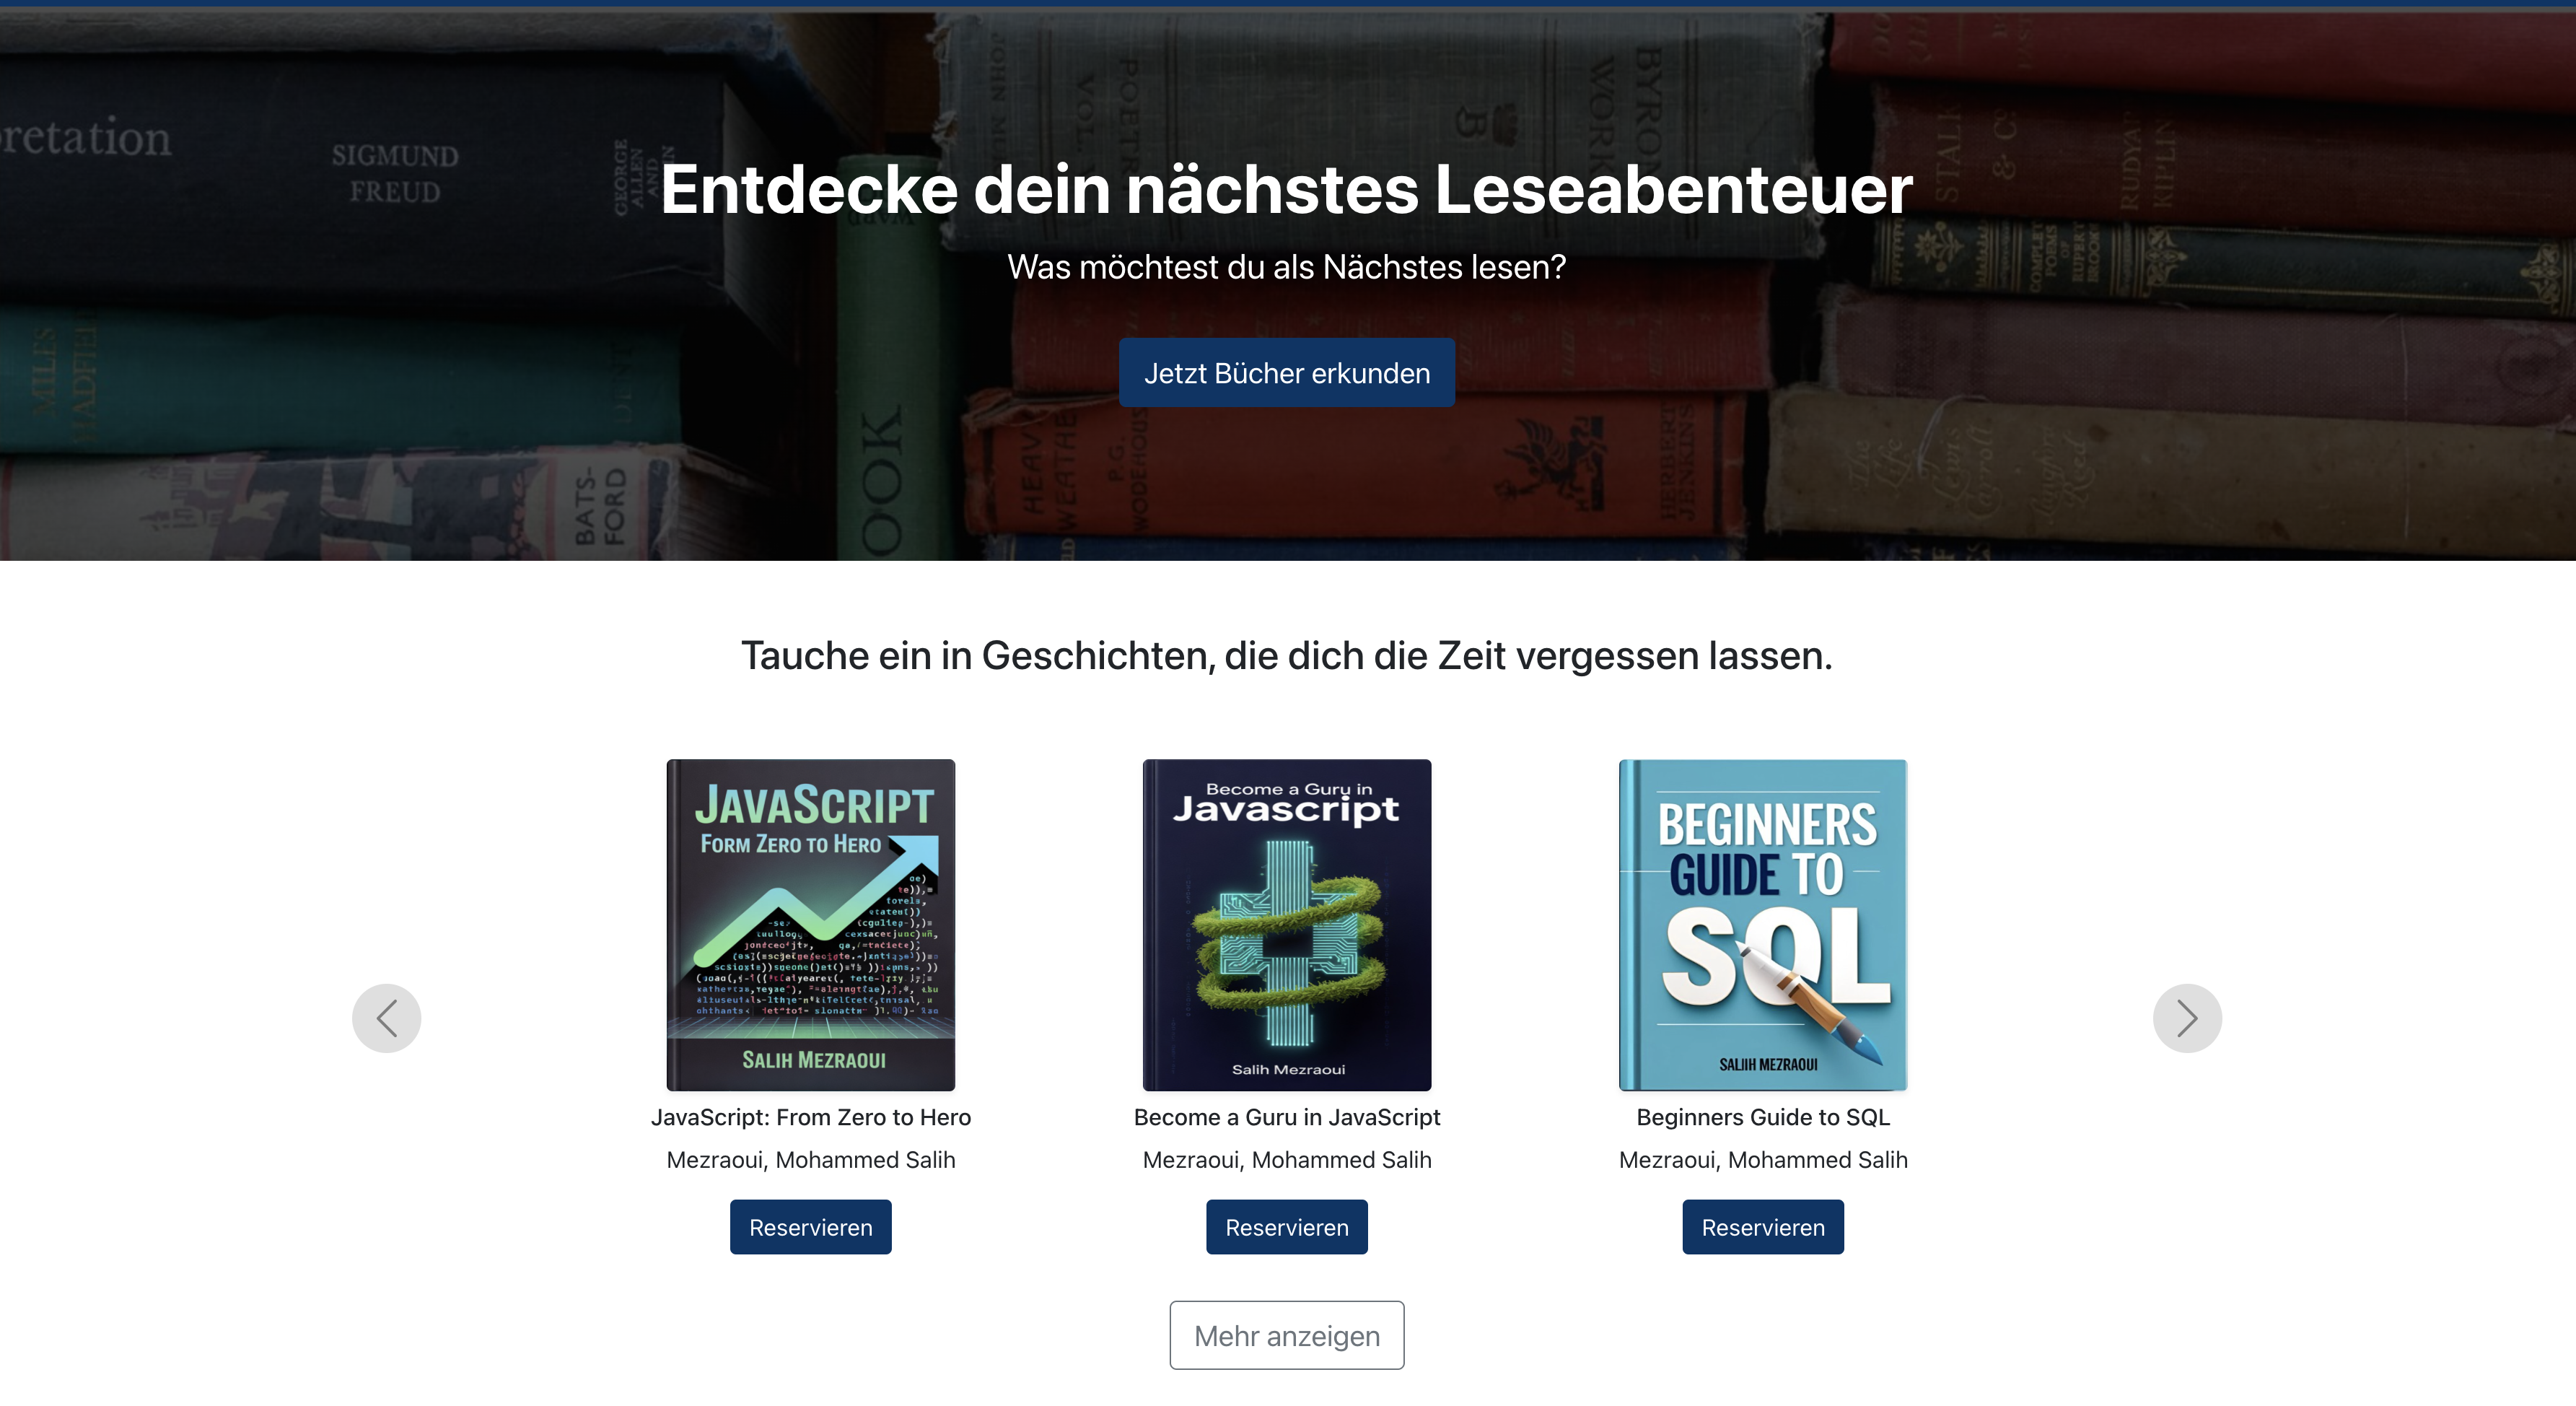
\includegraphics[width=1.0\textwidth]{images/UI-screenshots/Carousel_and_BookBrowser.png}%\subsection{Startseite (Main Page)}
	\caption{Karussell und Buch-Browser-Schaltfläche}
	\label{fig:Carousel_and_BookBrowser}%\subsubsection{Karussell (Carousel)}
\end{figure}

\subsection*{}\index{Link zur Bibliotheksdienste}

Die folgende Abbildung \ref{fig:Bibliotheksdienste-Link} zeigt einen Link zu den Bibliotheksdiensten, der angezeigt wird, wenn der Benutzer angemeldet ist. Andernfalls erscheint die Option ‚Registrieren‘.

\begin{figure}[H]
	\centering
	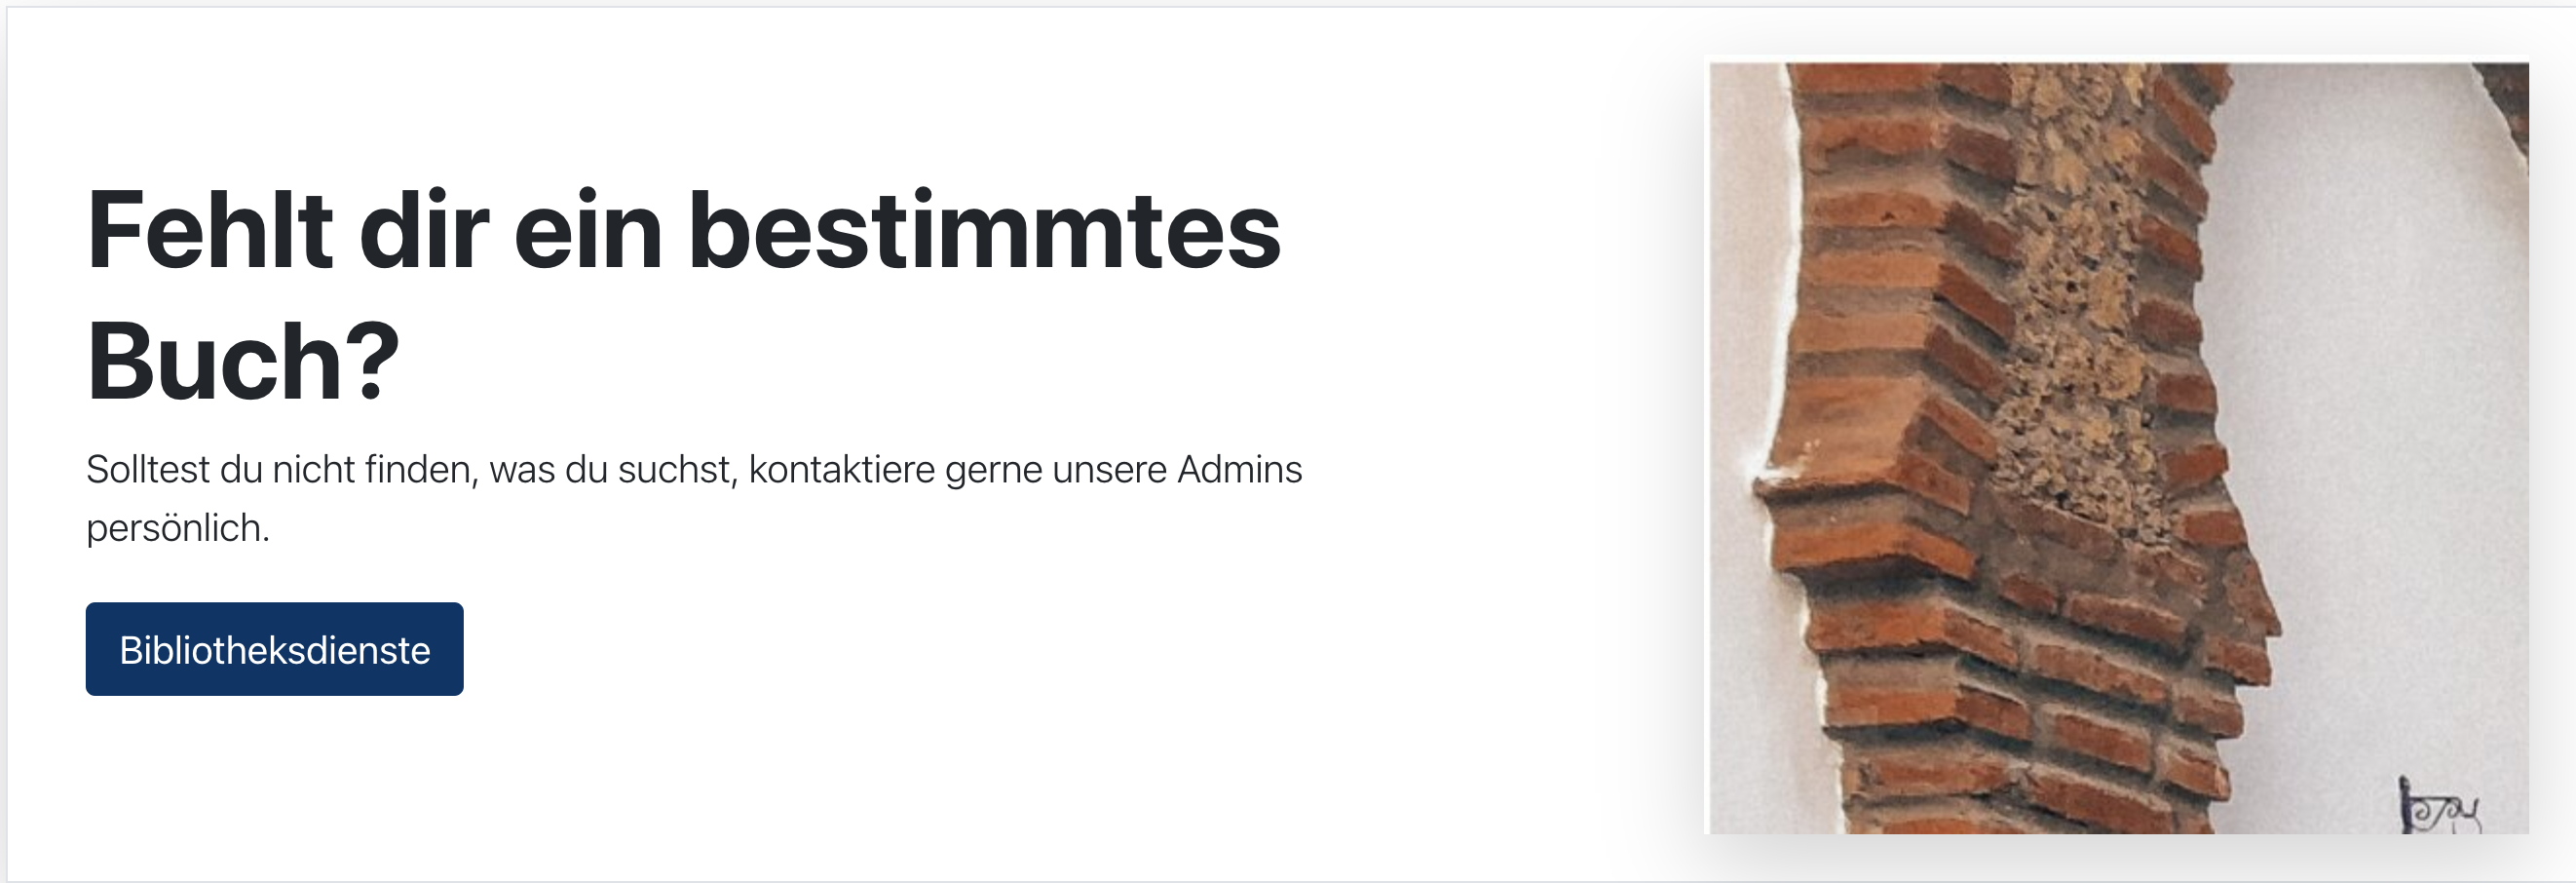
\includegraphics[width=1.0\textwidth]{images/UI-screenshots/Bibliotheksdienste-Link.png}%\subsection{Startseite (Main Page)}
	\caption{Karussell und Buch-Browser-Schaltfläche}
	\label{fig:Bibliotheksdienste-Link}%\subsubsection{Karussell (Carousel)}
\end{figure}

\section{Seitenübersicht}
Dieser Abschnitt gibt einen Überblick über zentrale Benutzeroberflächen der Anwendung, insbesondere die Buchsuchseite und die Buchdetailseite, und beschreibt deren wichtigste Funktionselemente.

\subsection{Buchsuche}

Die untenstehende Abbildung  \ref{fig:Search-page} zeigt die Benutzeroberfläche der Suchseite. Sie enthält ein Suchfeld mit Schaltfläche sowie ein Dropdown-Menü zur Auswahl von Kategorien. Nutzer können entweder nach Stichwörtern, Kategorien oder einer Kombination aus beiden suchen. Die Suchergebnisse werden in paginierter Form dargestellt und beinhalten jeweils den Buchtitel, den Autor, eine Kurzbeschreibung sowie eine Schaltfläche zur Detailansicht des jeweiligen Buches.

\begin{figure}[H]
	\centering
	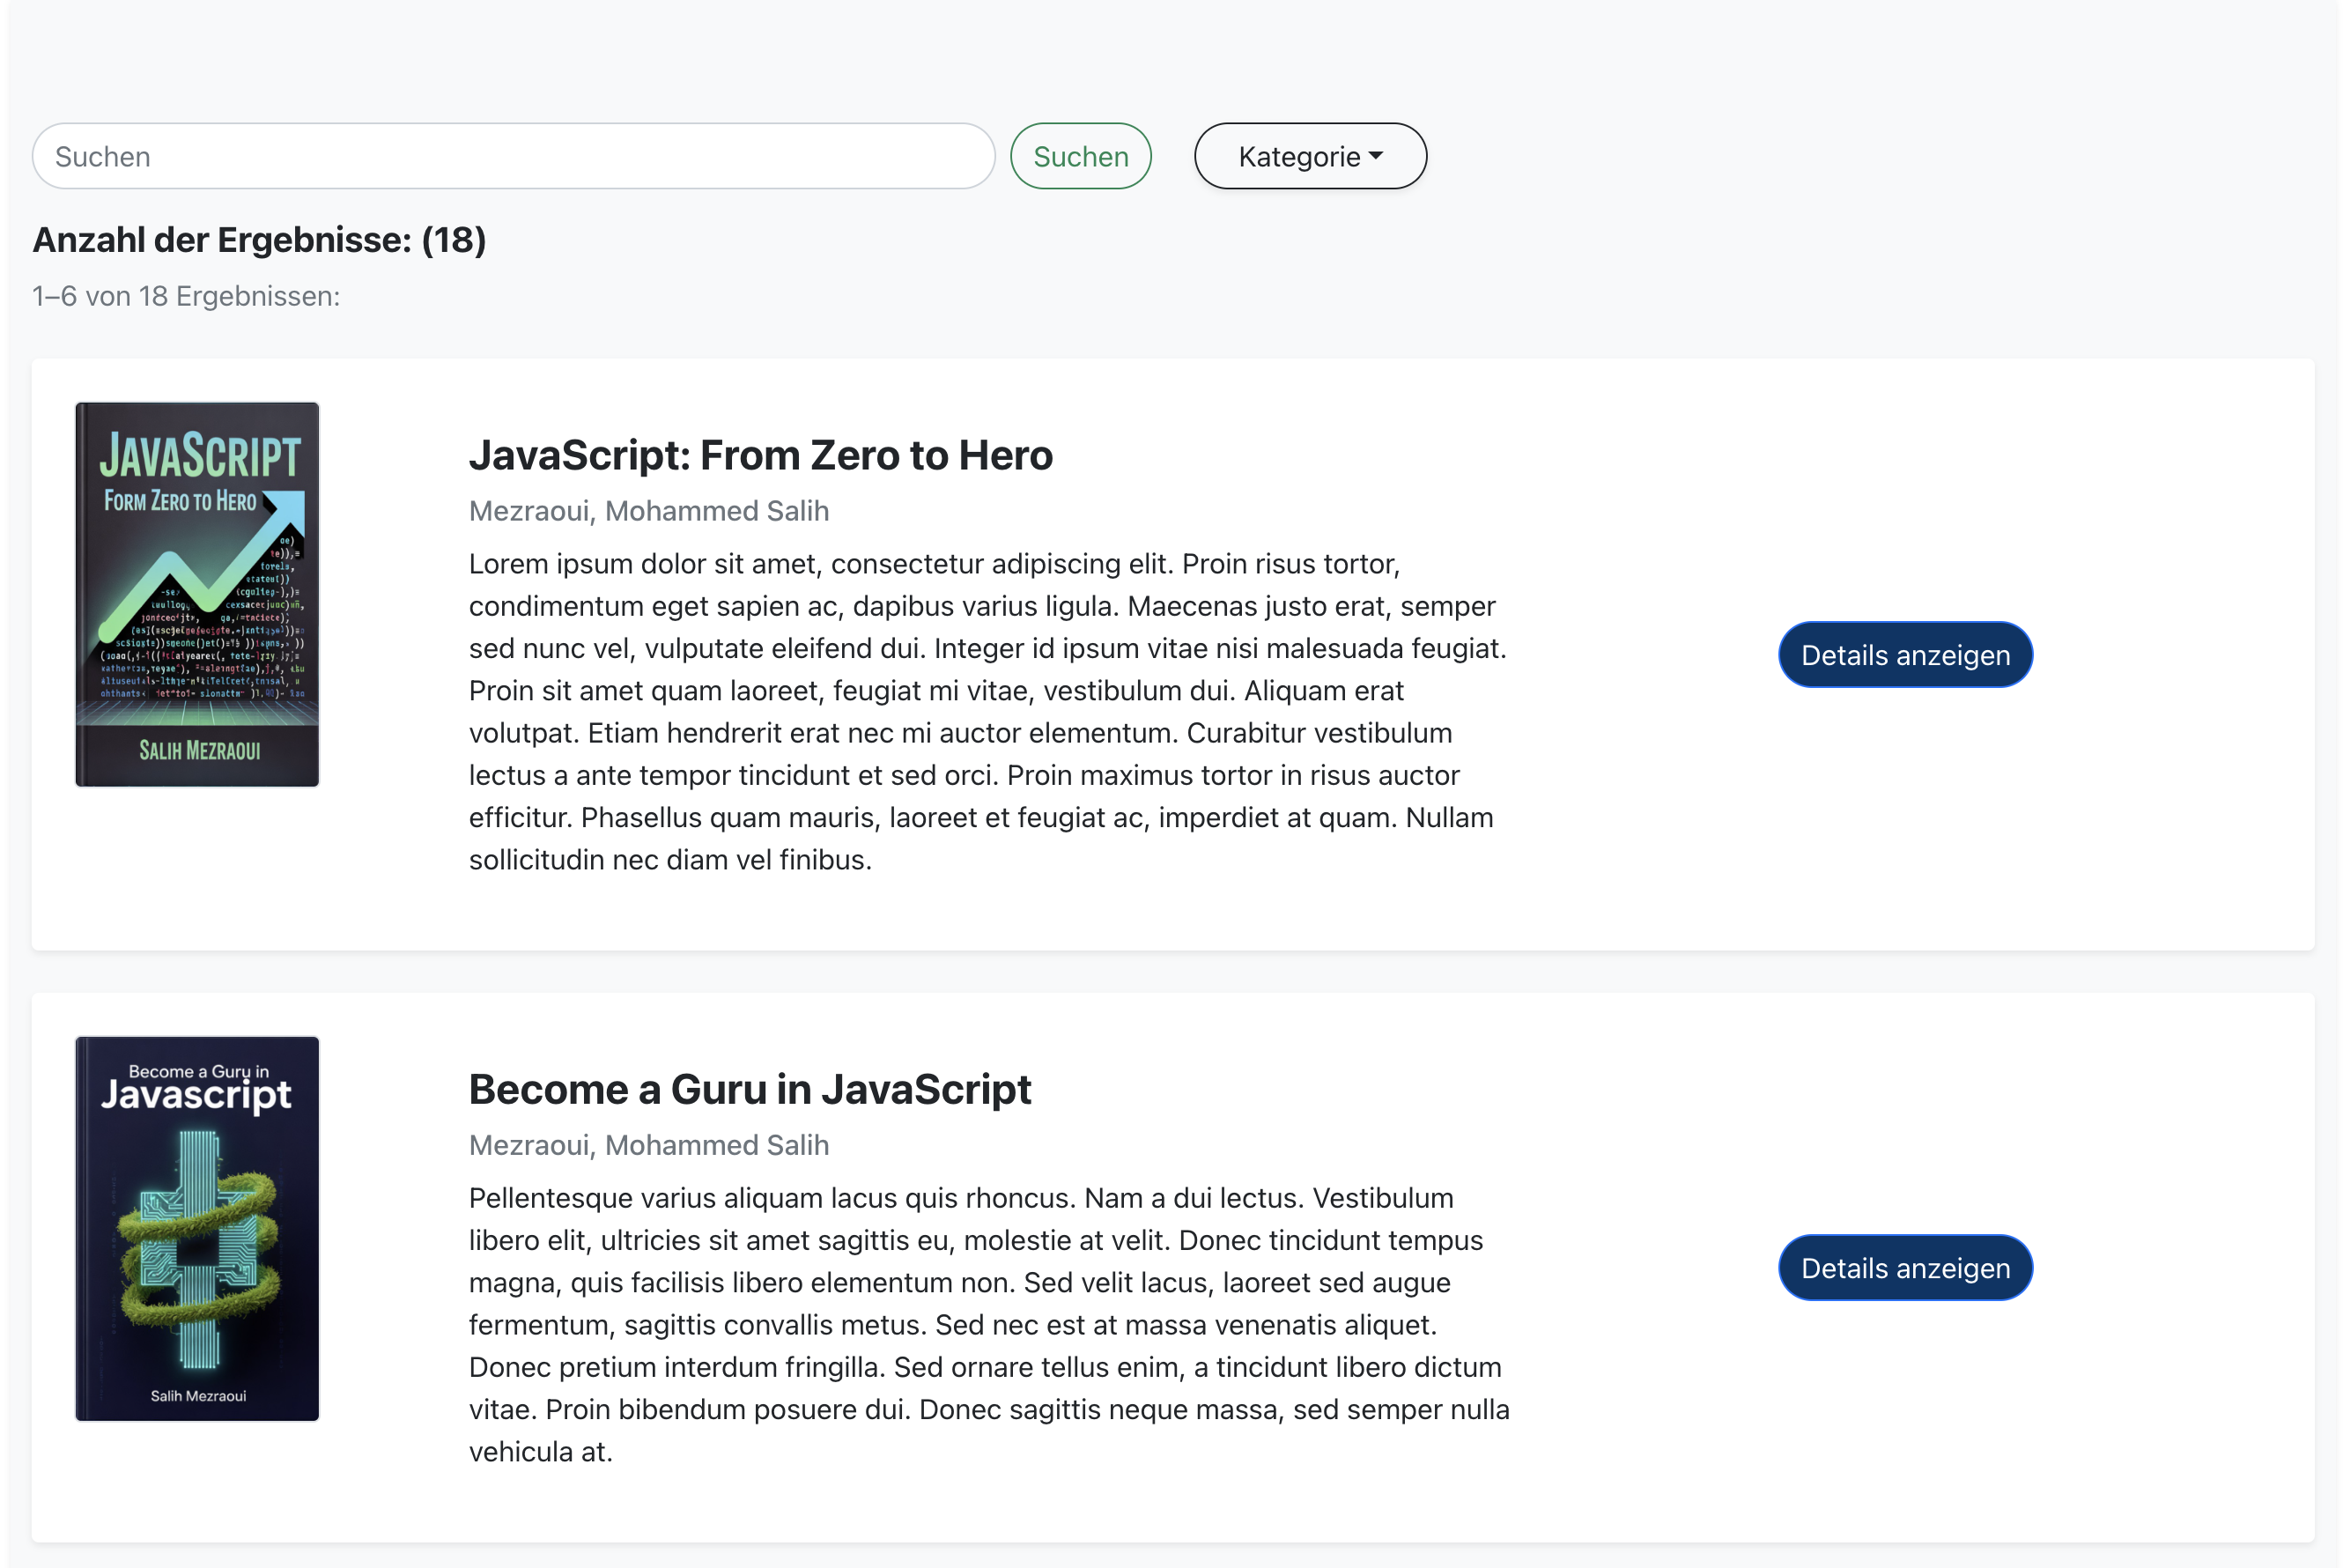
\includegraphics[width=1.0\textwidth]{images/UI-screenshots/Search-page.png}%\subsection{Startseite (Main Page)}
	\caption{Benutzeroberfläche der Suchseite}
	\label{fig:Search-page}
\end{figure}

\subsection{Buchseite}
Die untenstehende Abbildung  \ref{fig:Book-page} zeigt die Benutzeroberfläche der Buchseite. 

\begin{figure}[H]
	\centering
	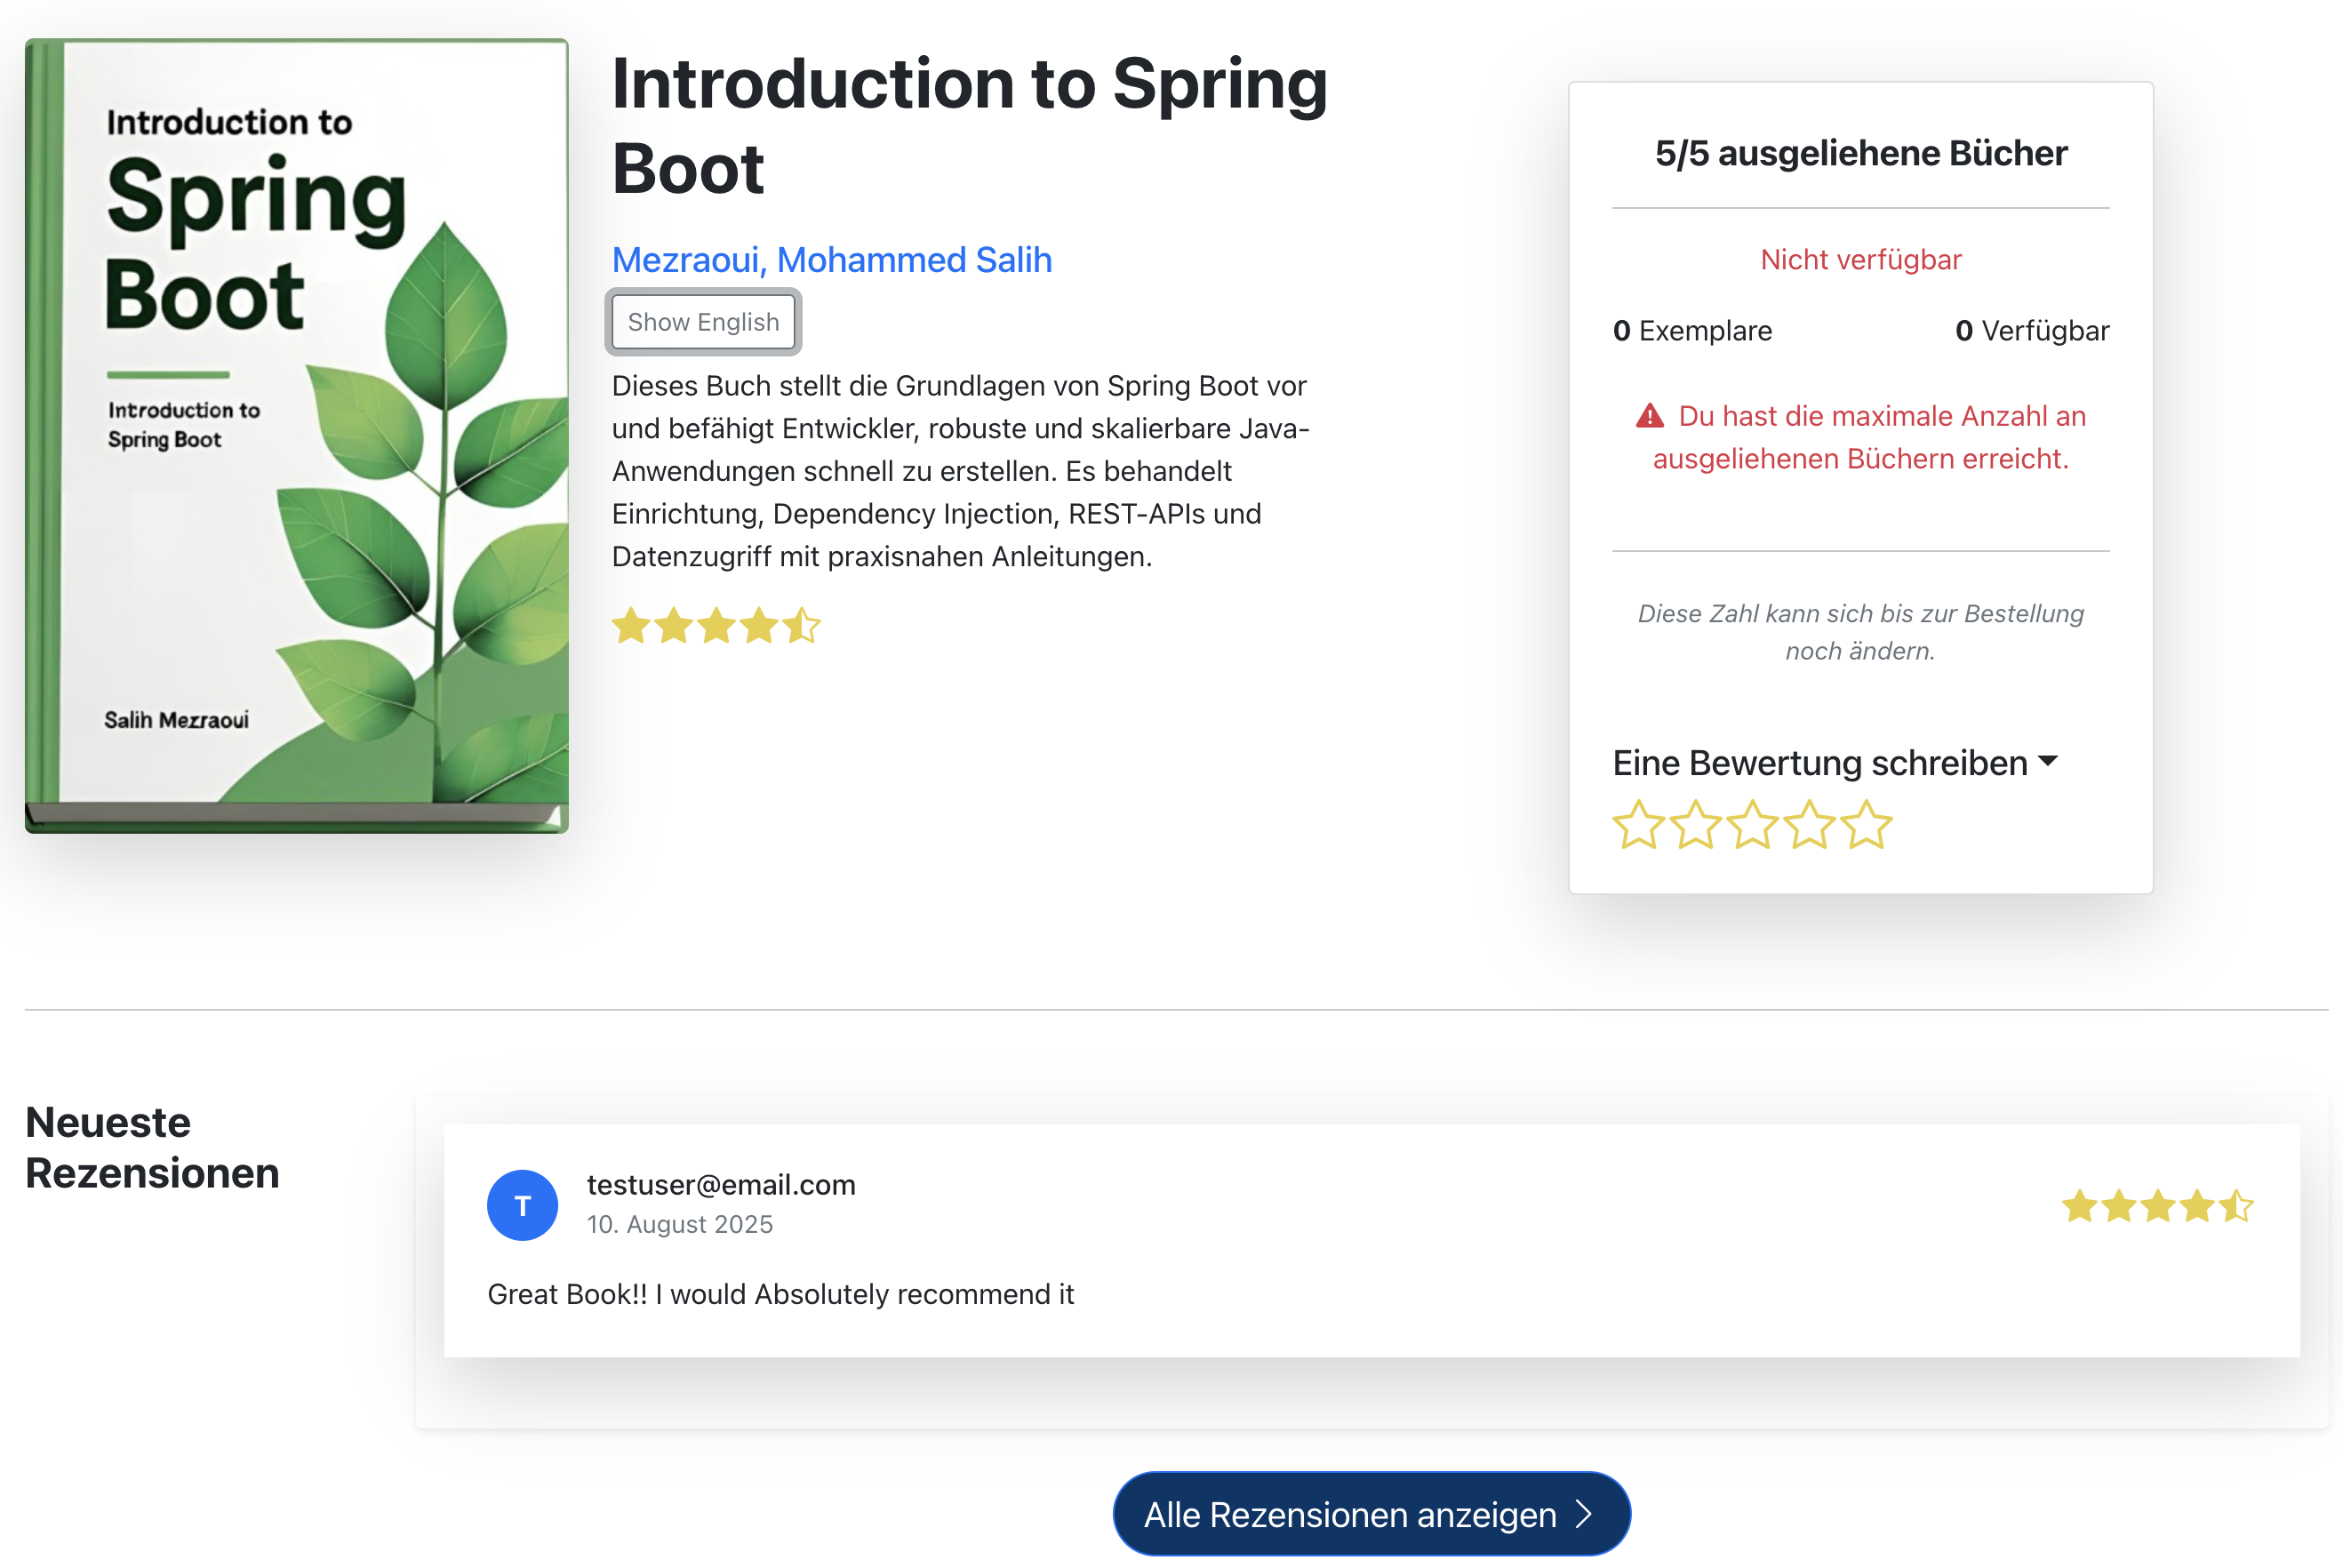
\includegraphics[width=1.0\textwidth]{images/UI-screenshots/Book-Page.png}
	\caption{Benutzeroberfläche der Buchseite}
	\label{fig:Book-page}
\end{figure}

\noindent Die Buchdetailseite stellt umfassende Informationen zu einem einzelnen Buch bereit und enthält folgende Elemente:
\begin{itemize}
	\item Darstellung des Buchcovers.
	\item Anzeige des Buchtitels und des Autors.
	\item Buchbeschreibung mit der Möglichkeit, zwischen deutscher und englischer Sprache zu wechseln, unabhängig von der Spracheinstellung der Gesamtanwendung.
	\item Bewertungssystem zur Anzeige der durchschnittlichen Nutzerbewertung.
	\item Rechte Seitenleiste mit folgenden Informationen:
	\begin{itemize}
		\item Anzahl der vom aktuellen Benutzer ausgeliehenen Exemplare,
		\item Anzahl der derzeit verfügbaren Exemplare,
		\item Gesamtanzahl der im Bestand befindlichen Exemplare.
	\end{itemize}
	\item Übersicht der Nutzerbewertungen zum Buch.
	\item Link zur vollständigen Liste aller Reviews.
\end{itemize}

\section{Bibliotheksaktivität}
In diesem Abschnitt werden die Funktionen zur Verwaltung aktueller und vergangener Ausleihen dargestellt.

\subsection{Ausleihen}
Die untenstehende Abbildung \ref{fig:Loans-Page} zeigt das Design der \texttt{Ausleihen} Seite. 

\begin{figure}[H]
	\centering
	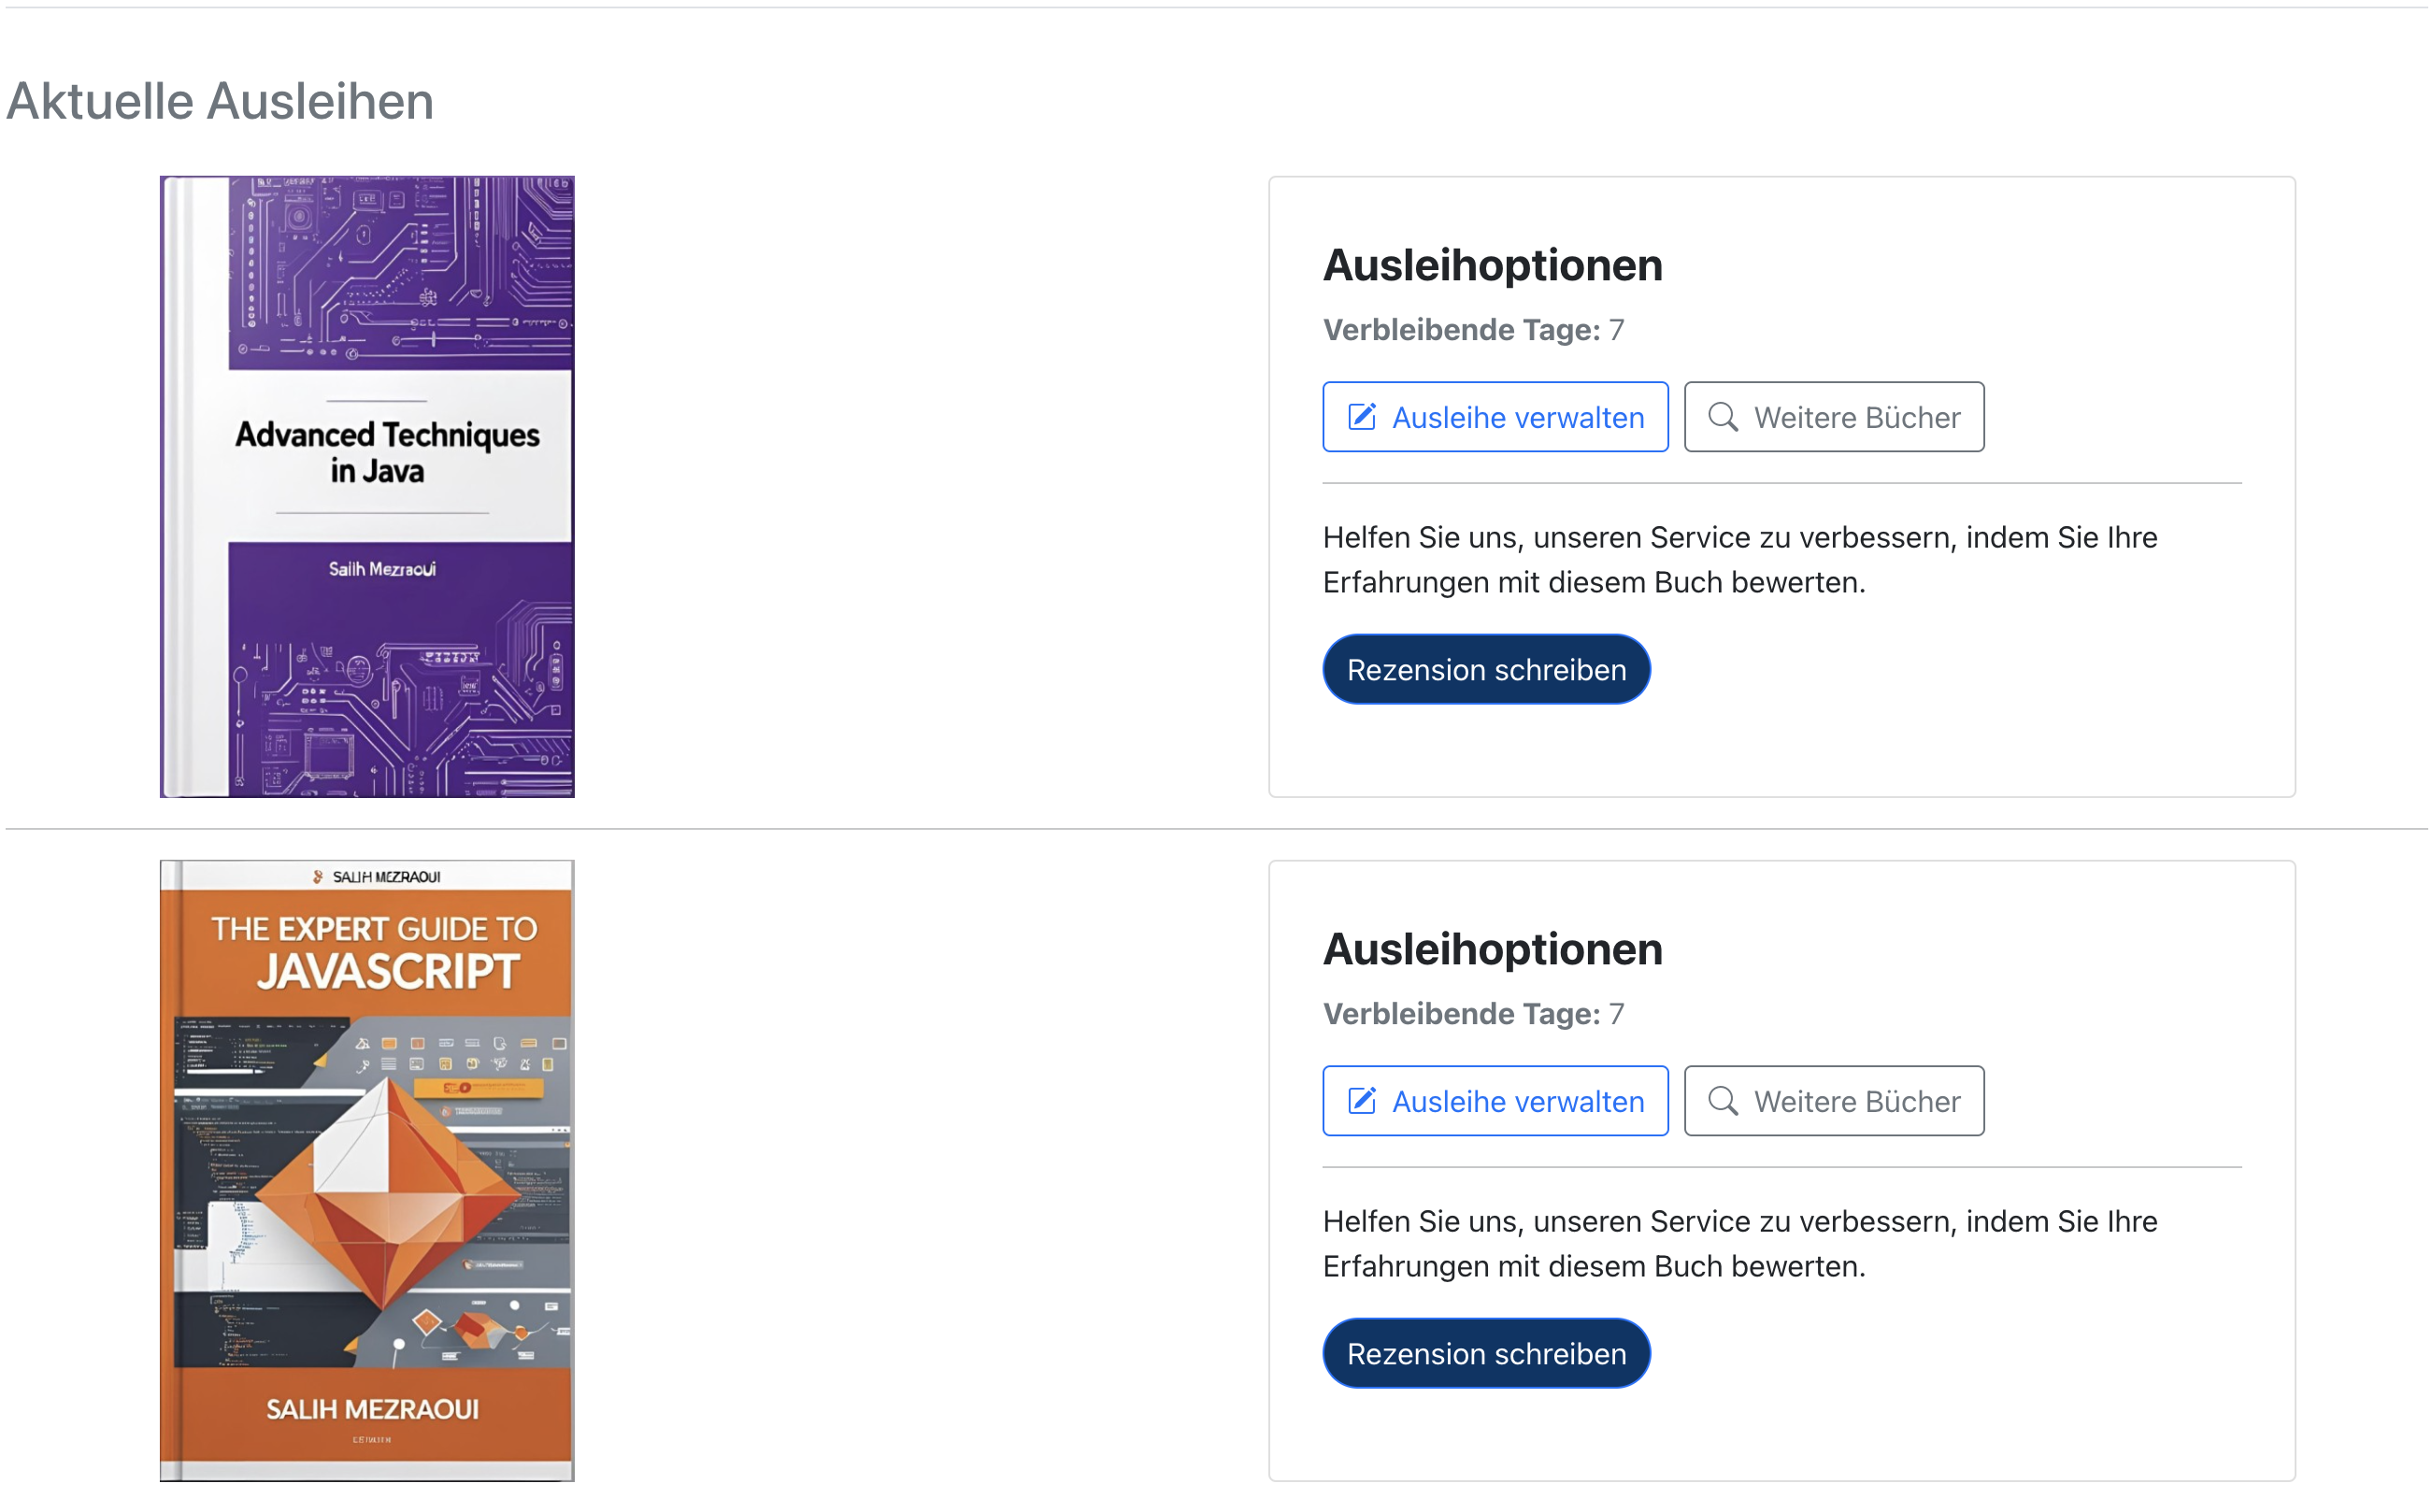
\includegraphics[width=1.0\textwidth]{images/UI-screenshots/Loans-Page.png}
	\caption{Benutzeroberfläche der Ausleihseite}
	\label{fig:Loans-Page}
\end{figure}

Die Ausleiheseite ermöglicht es Nutzerinnen und Nutzern, ihre aktuell ausgeliehenen Bücher zu verwalten. Sie enthält folgende Elemente:

\begin{itemize}
	\item Liste aller aktuell ausgeliehenen Bücher.
	\item Anzeige der verbleibenden Tage bis zur Rückgabe jedes Buches.
	\item Verwaltungsoptionen pro Buch:
	\begin{itemize}
		\item Rückgabe des Buches,
		\item Verlängerung der Leihfrist.
	\end{itemize}
	\item Schaltfläche zur Suche nach weiteren Büchern.
	\item Link zum Verfassen einer Rezension für das jeweilige Buch.
\end{itemize}

\subsection{Ausleihhistorie}
Die untenstehende Abbildung \ref{fig:Loans-History-Page} zeigt das Design der Seite \texttt{Ausleihverlauf}. Diese Seite enthält die Historie der vom Nutzer ausgeliehenen Bücher, einschließlich des Ausleih- und Rückgabedatums.

\begin{figure}[H]
	\centering
	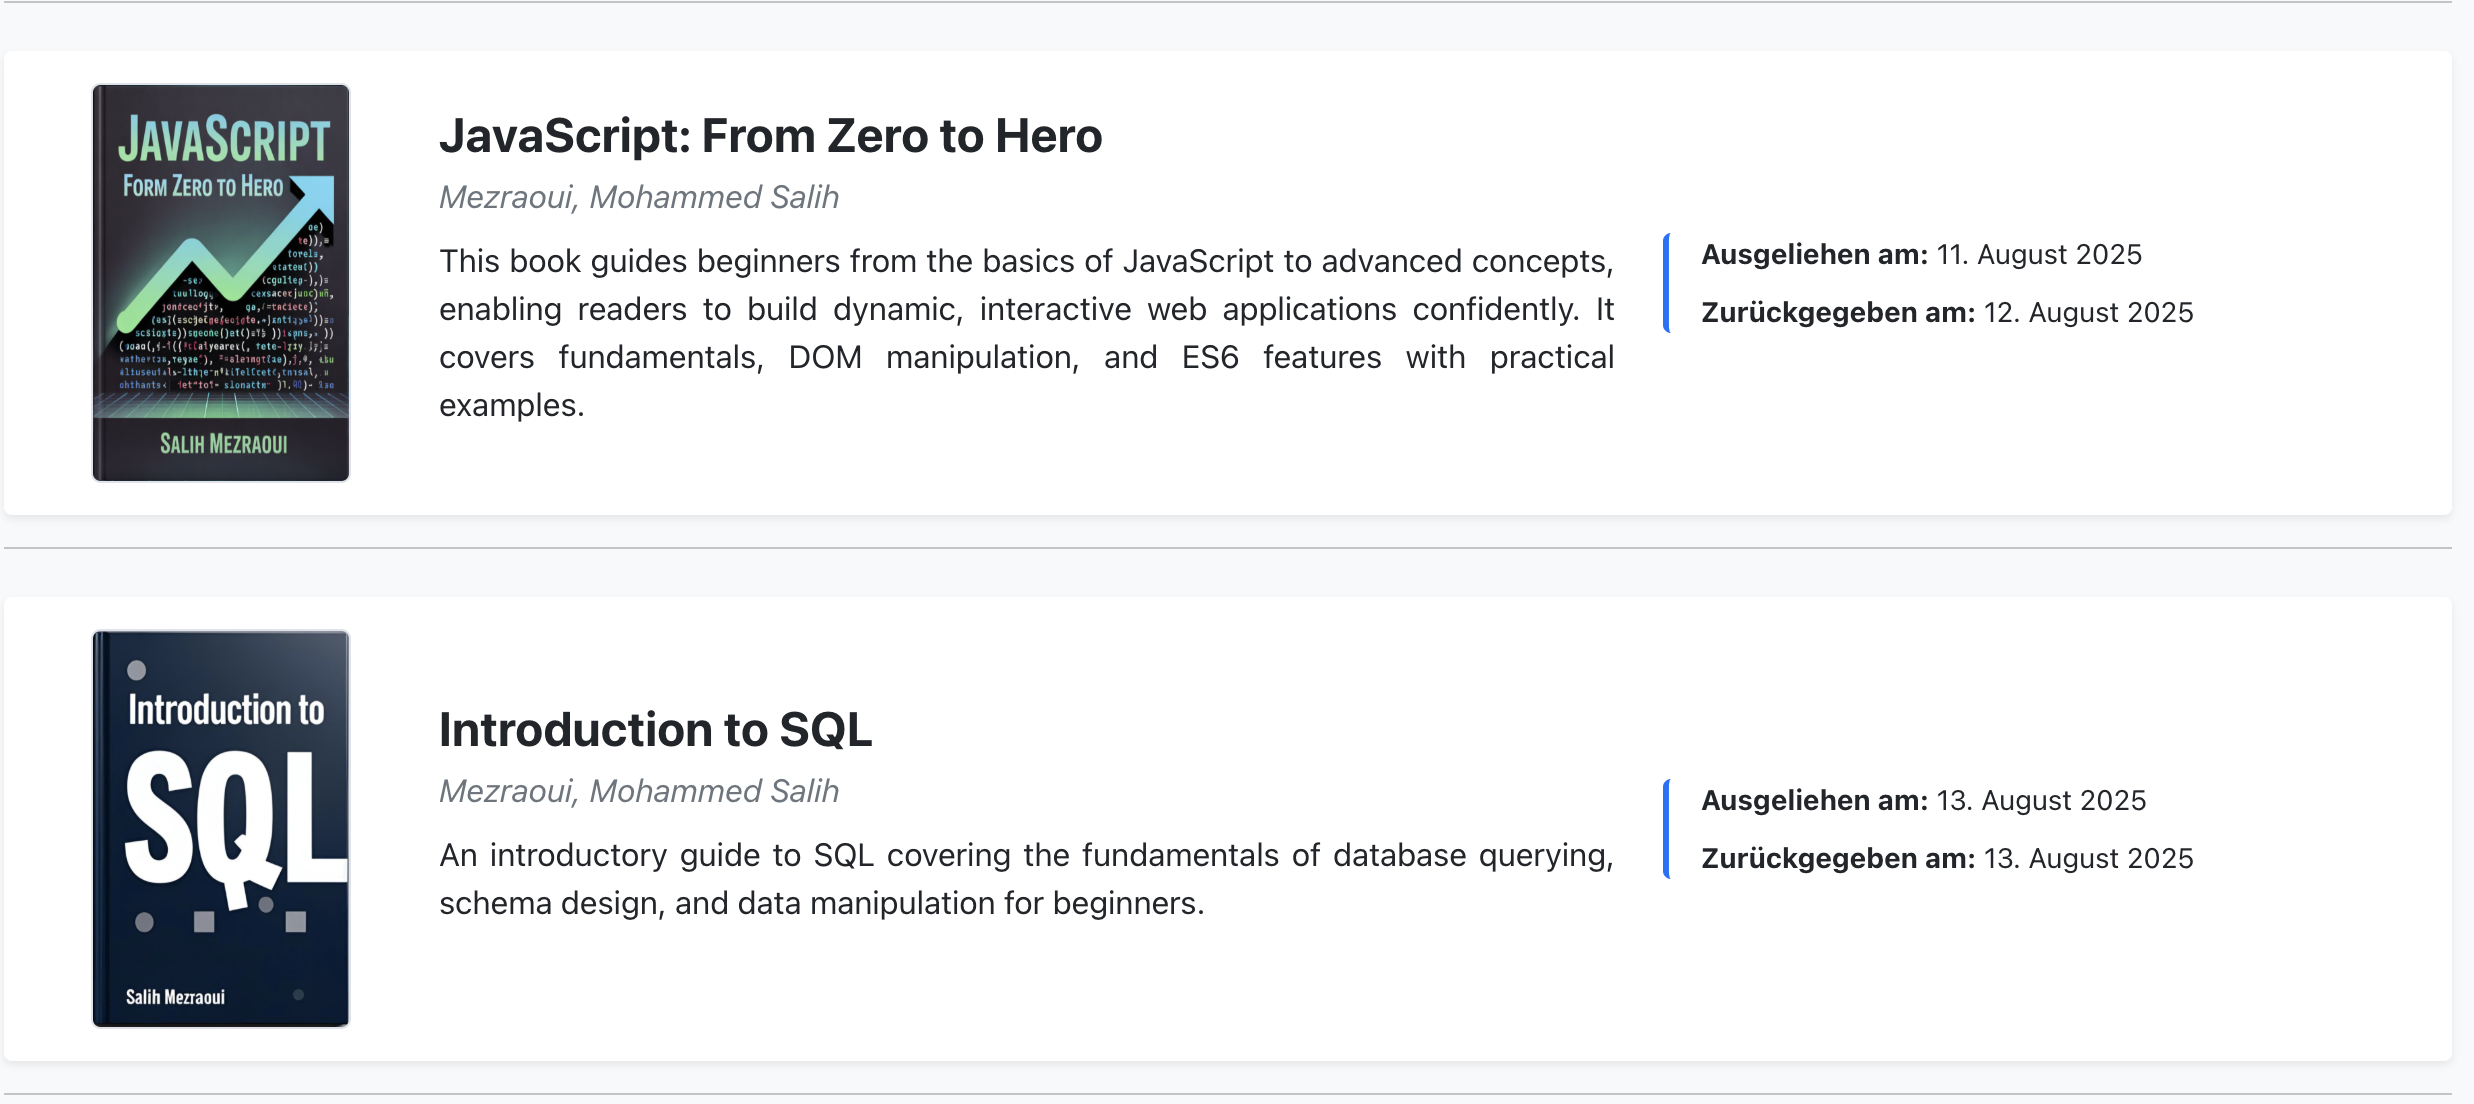
\includegraphics[width=1.0\textwidth]{images/UI-screenshots/Loans-History.png}
	\caption{Benutzeroberfläche der Ausleihverlaufsseite}%\subsection{Bibliotheksservice (Library Service)}
	\label{fig:Loans-History-Page}
\end{figure}

\section{Bibliotheksdienste}
In diesem Abschnitt werden die Bibliotheksdienste vorgestellt, insbesondere die Benutzeroberfläche zur Übermittlung von Anfragen sowie der persönliche Nachrichtenverlauf mit den jeweiligen Antworten.

\noindent Die folgende Abbildung \ref{fig:Message-Send} zeigt die Benutzeroberfläche, über die Benutzer einzelne Anfragen oder Nachrichten an die Administratoren der Bibliothek senden können.

\begin{figure}[H]
	\centering
	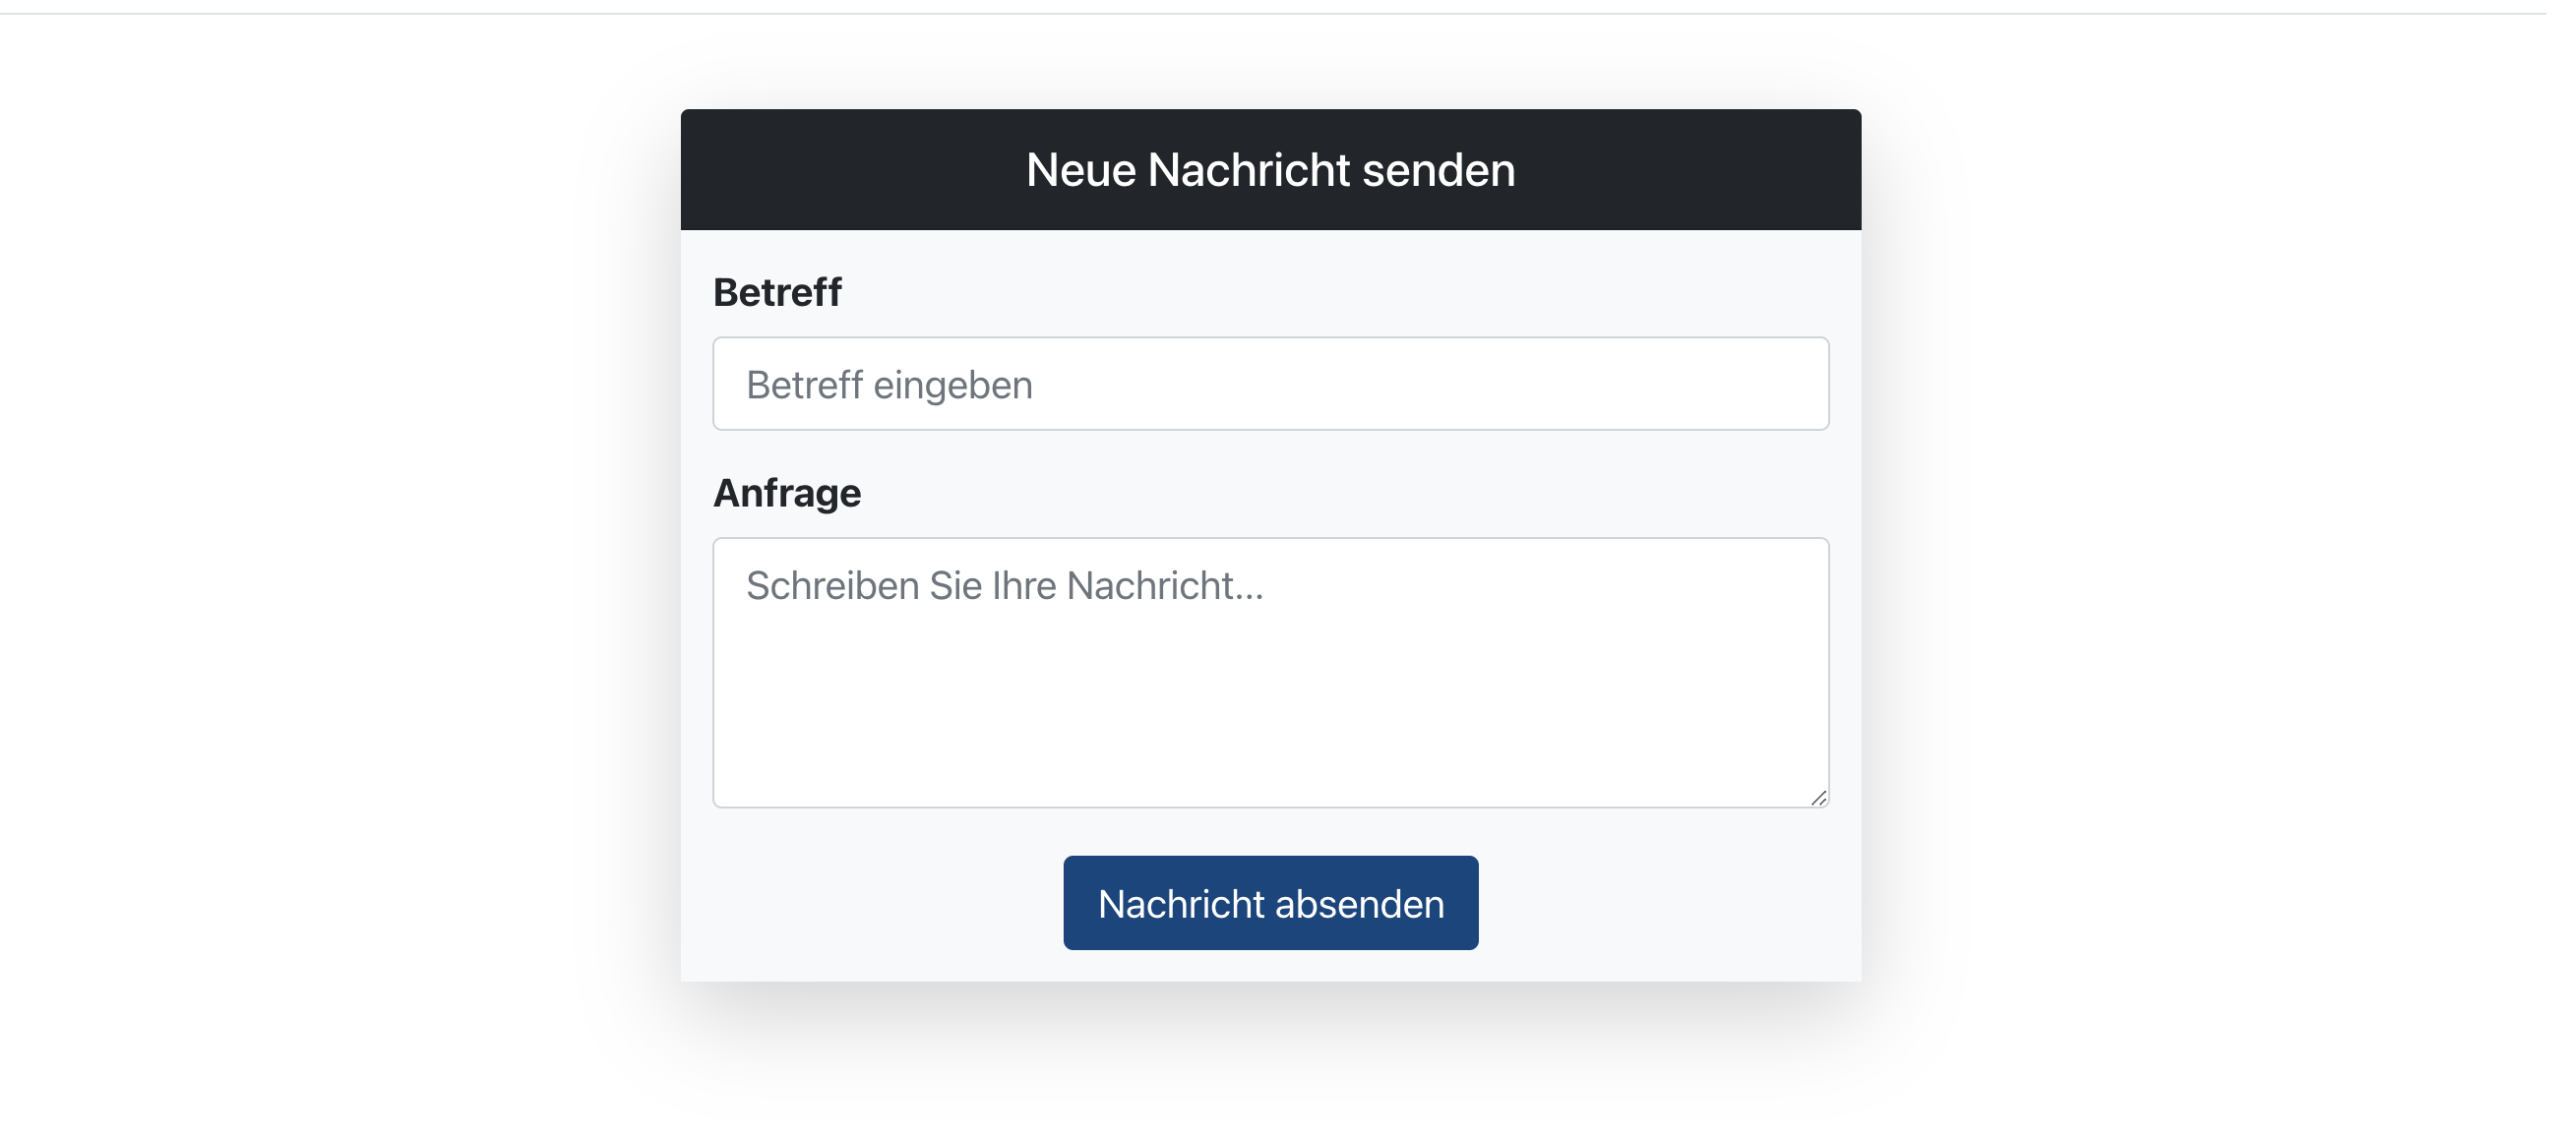
\includegraphics[width=1.0\textwidth]{images/UI-screenshots/Message-Send.png}
	\caption{Benutzeroberfläche zum Versenden von Anfragen}
	\label{fig:Message-Send}
\end{figure}

\noindent Die Abbildung \ref{fig:Messages-History} veranschaulicht den Verlauf sämtlicher ausgetauschter Nachrichten, einschließlich der gestellten Fragen und der dazugehörigen Antworten.

\begin{figure}[H]
	\centering
	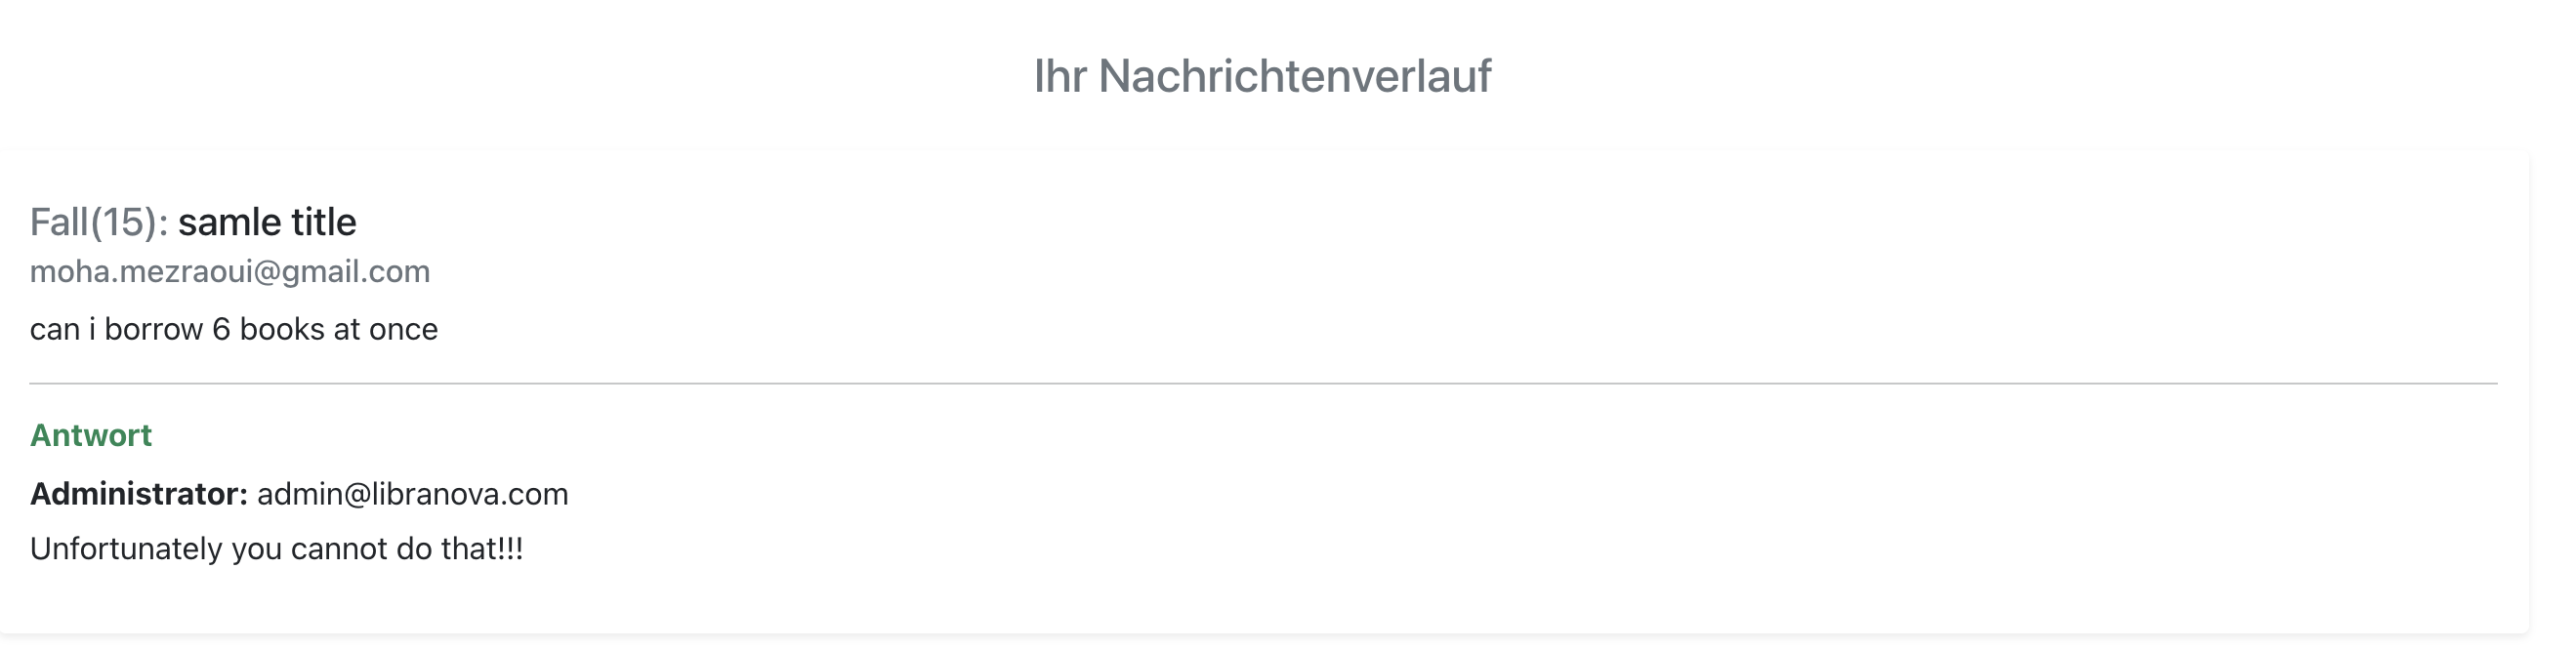
\includegraphics[width=1.0\textwidth]{images/UI-screenshots/Messages-History.png}
	\caption{Nachrichtenverlauf zwischen Nutzer und Bibliothek}
	\label{fig:Messages-History}
\end{figure}

\section{Bezahlungsseite}

In diesem Abschnitt wird die Benutzeroberfläche zur Verwaltung von Zahlungsinformationen und offenen Gebühren vorgestellt. \\

\noindent Abbildung \ref{fig:Outstanding-payment} zeigt das Layout, das angezeigt wird, wenn ein Benutzer ausstehende Zahlungen zu begleichen hat. 

\begin{figure}[H]
	\centering
	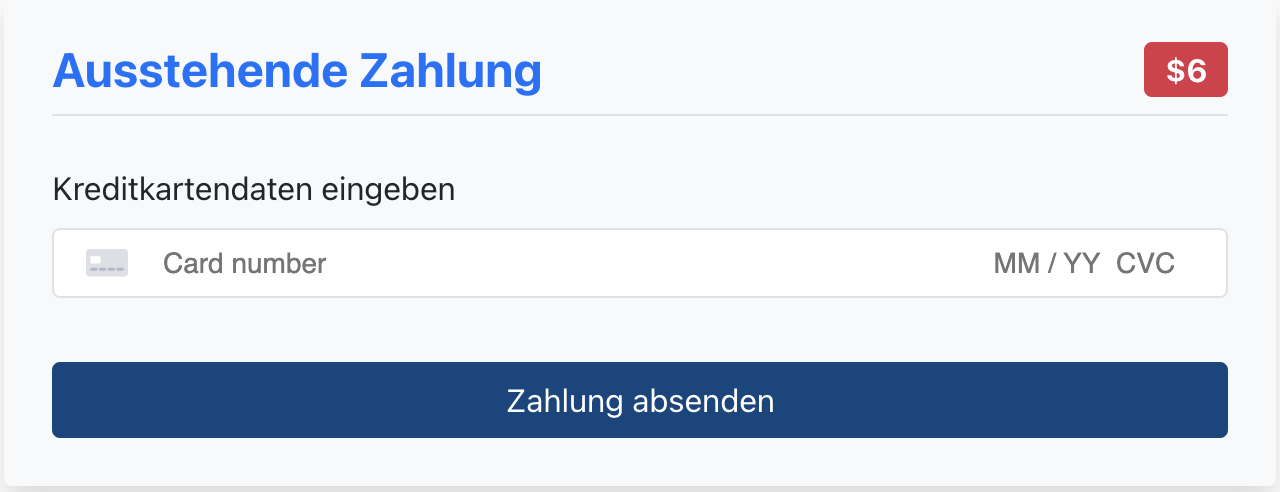
\includegraphics[width=1.0\textwidth]{images/UI-screenshots/Outstanding-payment.png}
	\caption{Benutzeroberfläche bei ausstehenden Zahlungen}
	\label{fig:Outstanding-payment}
\end{figure}

\noindent Wenn keine offenen Gebühren vorliegen, wird dem Nutzer die in Abbildung \ref{fig:No-Payment} dargestellte Ansicht präsentiert. Sie bestätigt, dass derzeit keine Zahlungen erforderlich sind.

\begin{figure}[H]
	\centering
	
\includegraphics[width=1.0\textwidth]{images/UI-screenshots/No-Payment.png}
	\caption{Benutzeroberfläche bei keinen offenen Zahlungen}
	\label{fig:No-Payment}
\end{figure}

\section{Admin-Bereich}

Der Admin-Bereich bietet eine dedizierte Oberfläche zur Verwaltung der Bibliotheksressourcen und zur Interaktion mit Benutzeranfragen. In diesem Abschnitt werden die Verwaltungsfunktionen dargestellt, die einem Administrator zur Verfügung stehen.

\subsection{Neues Buch hinzufügen}
\noindent Die erste Funktion (siehe \ref{fig:Add-New-Book})ermöglicht es dem Administrator, neue Bücher in das System aufzunehmen. Hierzu gibt er relevante Informationen wie Titel, Autor, Kategorie, eine kurze Beschreibung sowie die Anzahl der verfügbaren Exemplare an. Zusätzlich kann ein Bild des Buchcovers hochgeladen werden. Nach dem Ausfüllen der Felder wird durch Klicken auf die Schaltfläche \textit{"Buch hinzufügen"} ein neuer Eintrag erstellt.
\begin{figure}[H]
	\centering
	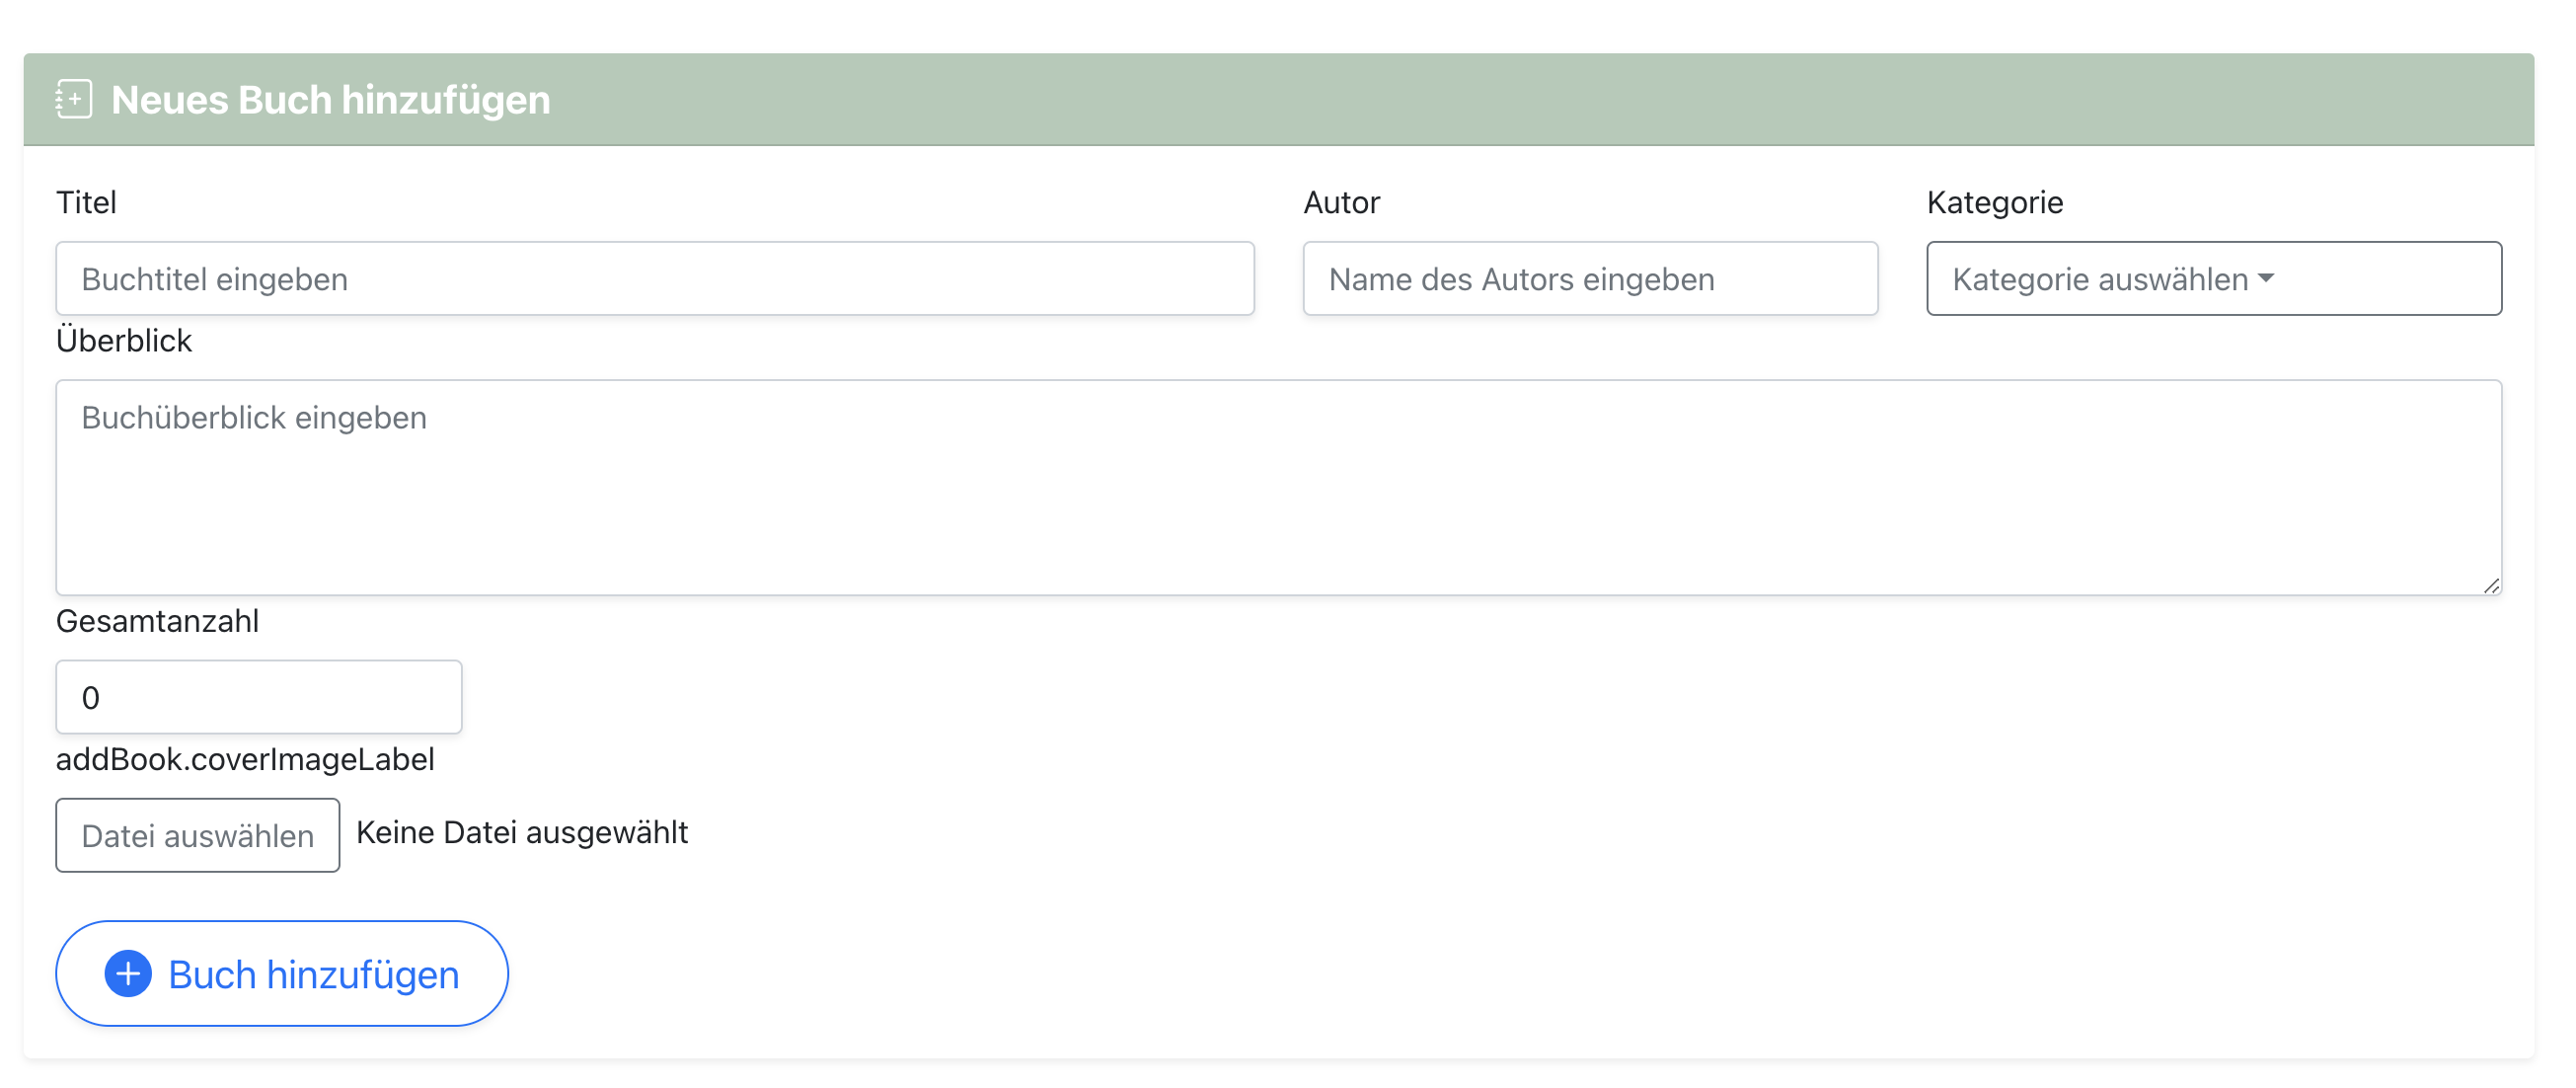
\includegraphics[width=1.0\textwidth]{images/UI-screenshots/Add-New-Book.png}
	\caption{Benutzeroberfläche bei keinen offenen Zahlungen}
	\label{fig:Add-New-Book}
\end{figure}

\subsection{Bücher verwalten}

\noindent Der Administrator kann bestehende Bücher verwalten, indem er die Anzahl der verfügbaren Exemplare anpasst oder Bücher vollständig aus dem System entfernt. Die folgende Abbildung \ref{fig:Manage-Books} zeigt die Verwaltungsoberfläche, über die solche Änderungen vorgenommen werden können.

\begin{figure}[H]
	\centering
	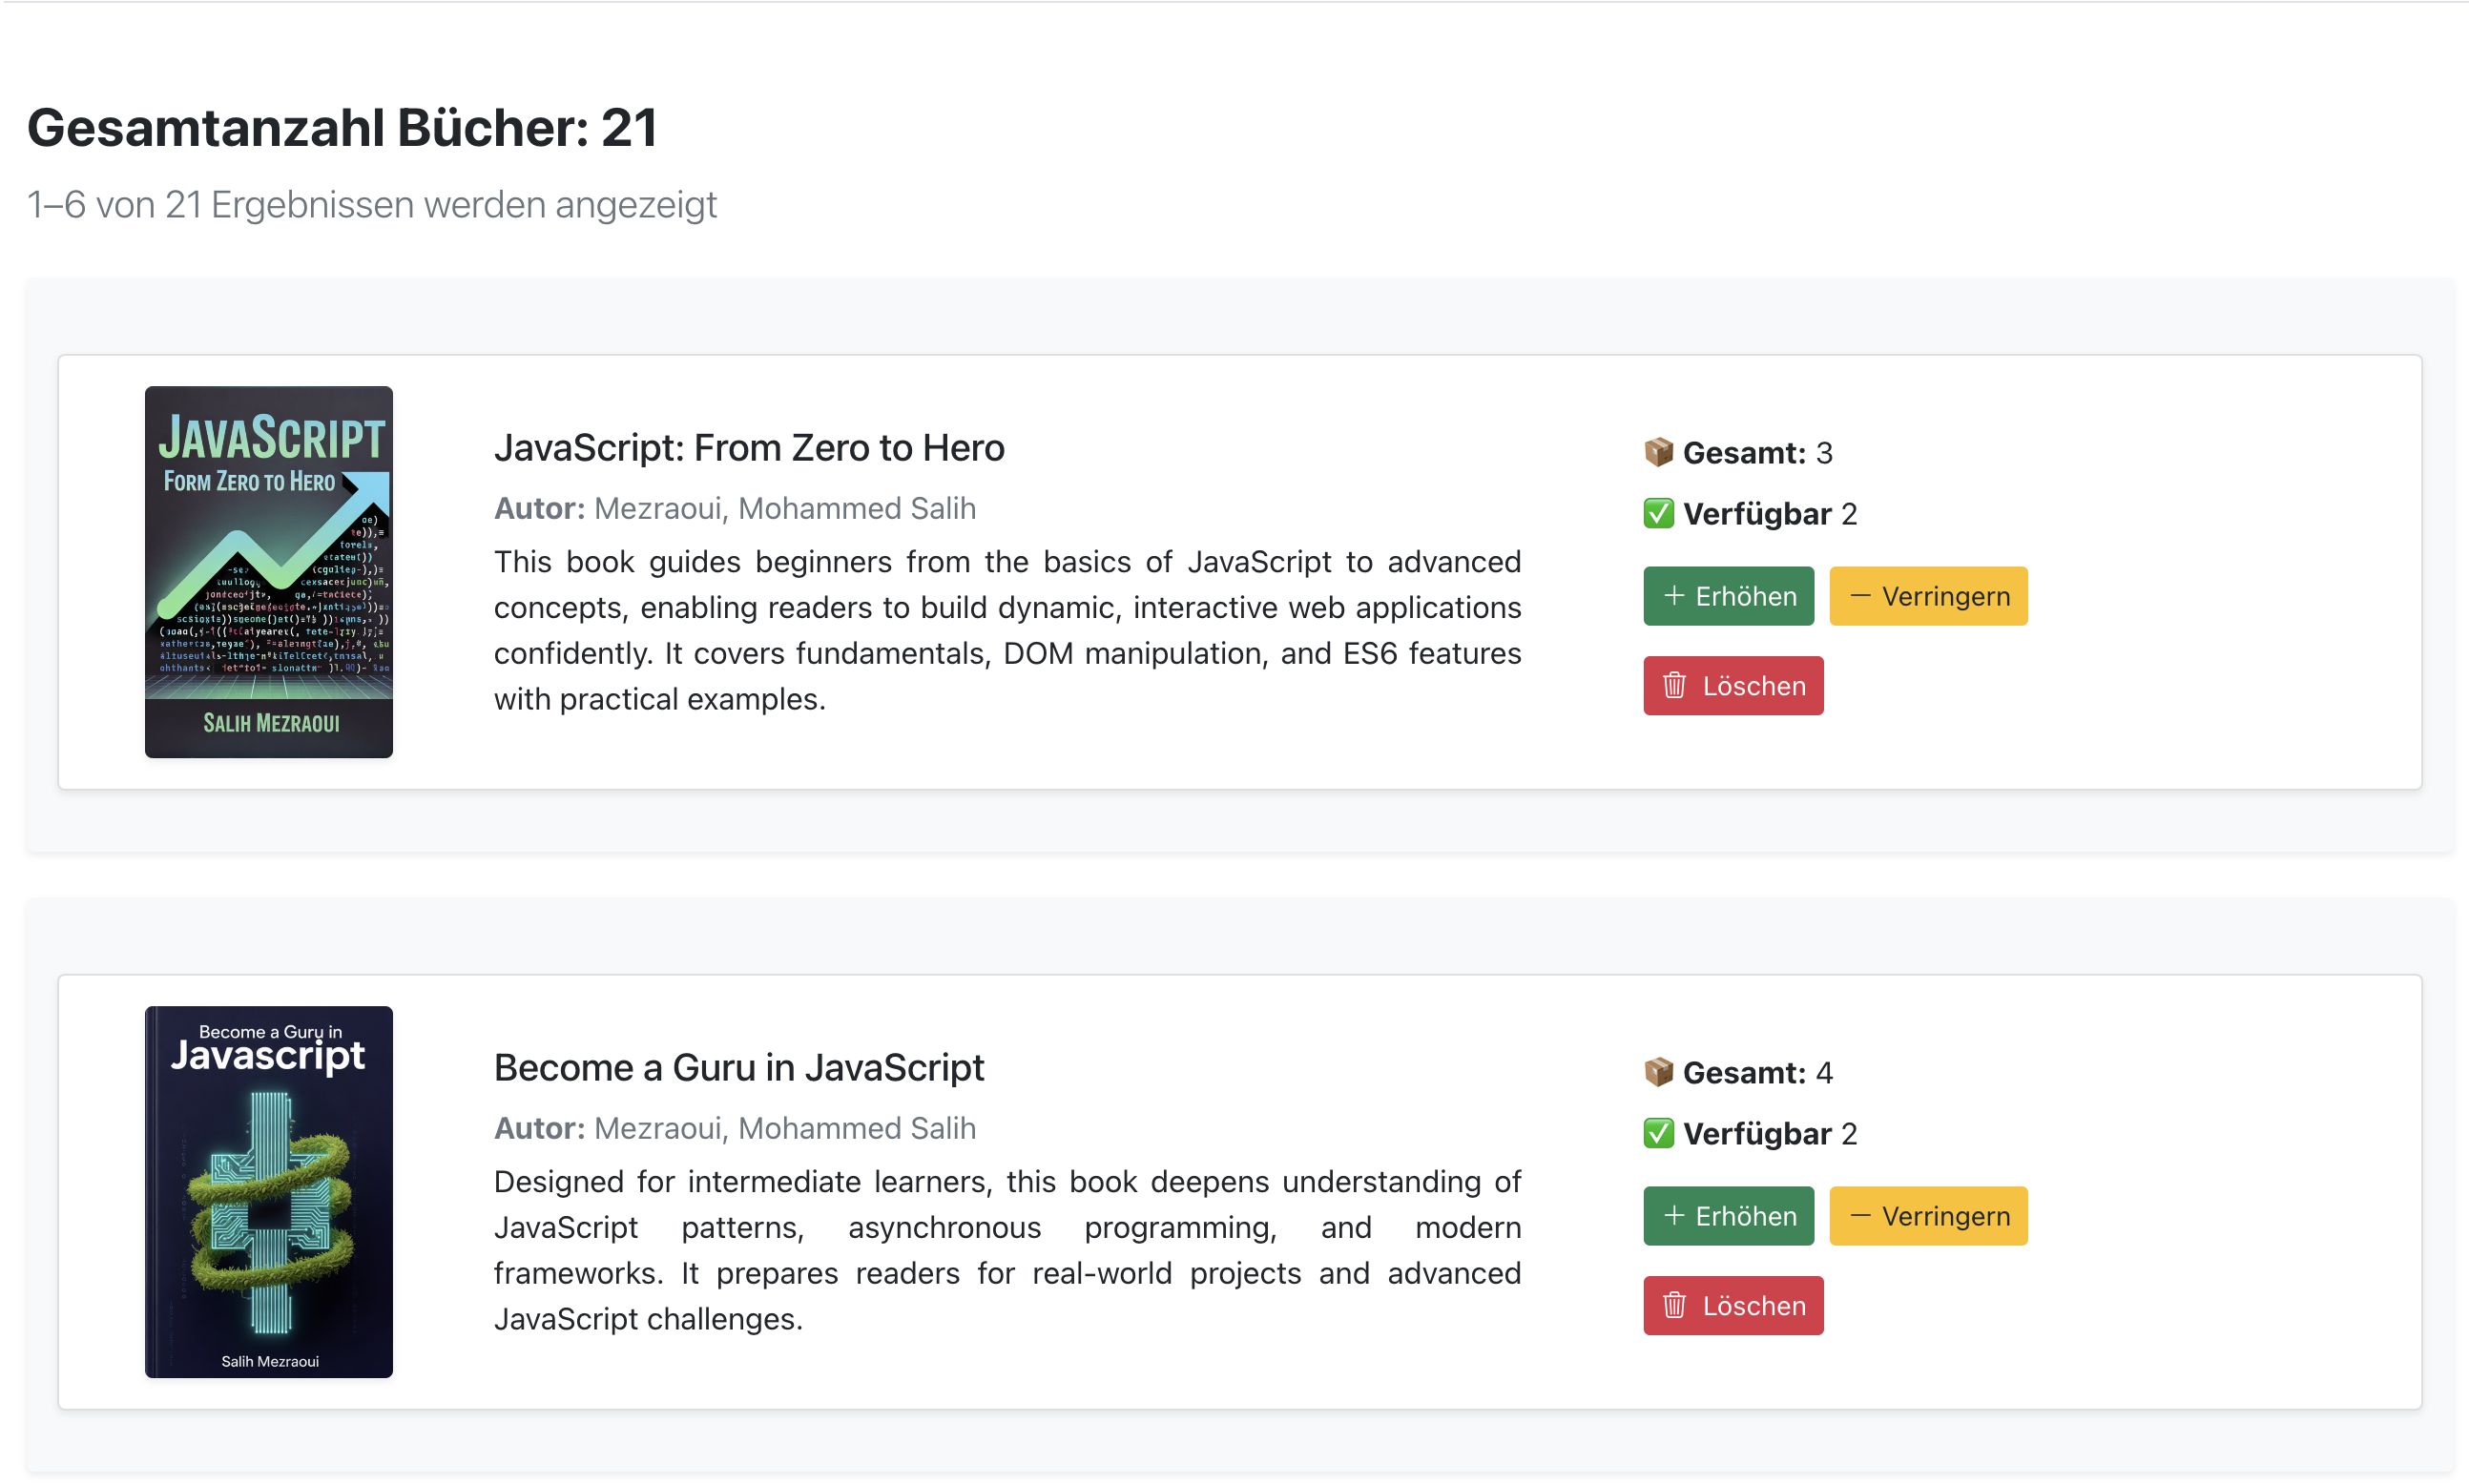
\includegraphics[width=1.0\textwidth]{images/UI-screenshots/Manage-Books.png}
	\caption{Benutzeroberfläche bei keinen offenen Zahlungen}
	\label{fig:Manage-Books}
\end{figure}
\subsection{Nachrichten}

\noindent In diesem Bereich kann der Administrator auf Anfragen von Benutzern antworten. Die Benutzerfrage wird angezeigt und kann direkt über das vorgesehene Textfeld beantwortet werden. Eine Schaltfläche ermöglicht das Senden der Antwort. Die Abbildung \ref{fig:Messages-Responses} zeigt die zugehörige Benutzeroberfläche.

\begin{figure}[H]
	\centering
	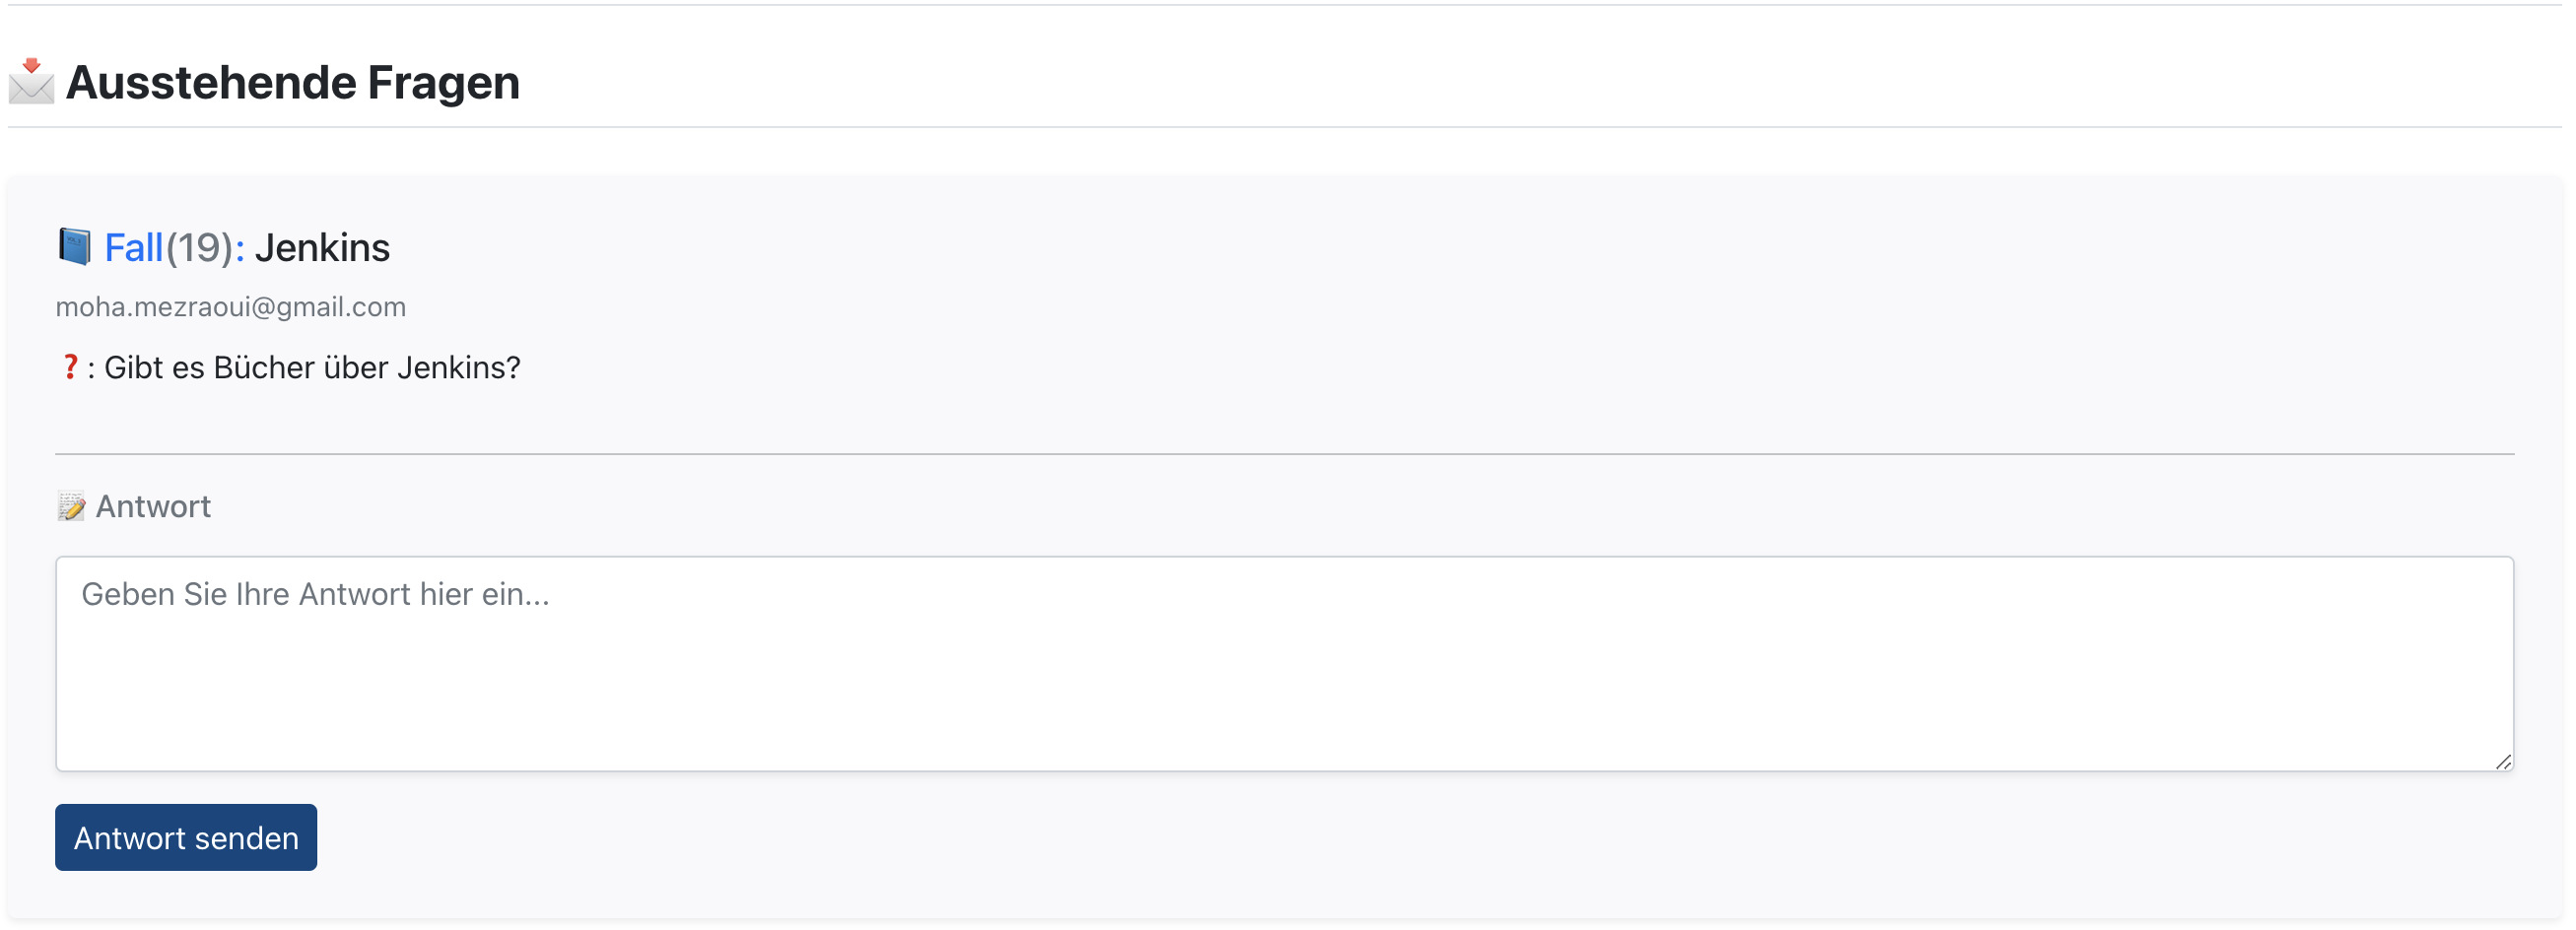
\includegraphics[width=1.0\textwidth]{images/UI-screenshots/Messages-Responses.png}
	\caption{Benutzeroberfläche bei keinen offenen Zahlungen}
	\label{fig:Messages-Responses}
\end{figure}





















\chapter{Zusammenfassung und Ausblick}

Diese Dokumentation hat die Konzeption, Implementierung und Analyse der Full-Stack-Bibliotheksmanagement-Anwendung „LibraNova“ umfassend dargestellt. Ziel des Projekts war es, eine moderne, benutzerfreundliche und sichere Plattform zu entwickeln, die den Anforderungen der Bibliotheksnutzer und Administratoren gerecht wird. Mit bewährten Technologien wie Spring Boot im Backend, React mit TypeScript im Frontend sowie einer Sicherheitsarchitektur mit Okta, JWT, OAuth2 und OpenID Connect konnte eine skalierbare und wartbare Lösung realisiert werden.

Die klare Trennung von Backend und Frontend sowie moderne Frameworks ermöglichten eine effiziente Entwicklung. Spring Security in Verbindung mit Okta sorgt für einen robusten Authentifizierungs- und Autorisierungsmechanismus, der die Sicherheit sensibler Daten gewährleistet. Die Integration von Redux im Frontend unterstützt ein effektives State-Management für eine reaktive und performante Benutzeroberfläche.

Die Anwendung umfasst Kernfunktionen zur Buchsuche, Ausleihe und Bewertung sowie administrative Werkzeuge zur Verwaltung des Buchkatalogs und der Nutzeranfragen. Die Qualitätssicherung erfolgte mit JUnit, Mockito und React Testing Library, um Backend- und Frontend-Komponenten systematisch zu testen und die Stabilität der Anwendung sicherzustellen. Postman diente als praktisches API-Testtool und ergänzte den Entwicklungsprozess.

Zukünftige Arbeiten könnten Cloud-Bereitstellung mit CI/CD-Pipelines, erweiterte Testabdeckung sowie Funktionen wie Benachrichtigungen oder personalisierte Empfehlungen umfassen. Die modulare Architektur erlaubt eine flexible Anpassung von LibraNova an unterschiedliche Bibliotheksanforderungen.

Insgesamt bietet LibraNova eine zeitgemäße Lösung, die den digitalen Wandel im Bibliotheksmanagement unterstützt und die Nutzererfahrung durch intuitive Bedienung und sichere Prozesse verbessert. Diese Dokumentation bildet eine Grundlage für weitere Entwicklungen und zeigt, wie moderne Webtechnologien effektiv kombiniert werden können, um praxisnahe und nachhaltige Anwendungen zu schaffen.


%------------------ Literaturverzeichnis & Index -------------------------------
\backmatter
\bibliography{literatur}								% Literaturverzeichnis (literatur.bib)
\printindex												% Index (optional)


%------------------ Anhänge ----------------------------------------------------
\begin{appendix}
	\include{chapters/Abkürzungsverzeichnis}							% Glossar (optional)
	\chapter{Selbstständigkeitserklärung}

\begin{description}


\item[$\Box$] Diese Arbeit wurde als Gruppenarbeit angefertigt. Meinen Anteil habe ich selbstständig verfasst und keine anderen als die angegebenen Quellen und Hilfsmittel verwendet.\\

Namen der Mitverfasser: \\

Imad-Eddine ABDESSAMI,
Mohammed Salih MEZRAOUI
\vspace{3cm}


\begin{minipage}[t]{3cm}
	\rule{3cm}{0.5pt}
	Datum
\end{minipage}
\hfill
\begin{minipage}[t]{9cm}
	\rule{9cm}{0.5pt}
	Unterschrift der Kandidatin/des Kandidaten
\end{minipage}


\end{description}

\vspace{2cm}

\begin{minipage}[t]{3cm}
	\rule{3cm}{0.5pt}
	Datum
\end{minipage}
\hfill
\begin{minipage}[t]{9cm}
	\rule{9cm}{0.5pt}
	Unterschrift der Kandidatin/des Kandidaten
\end{minipage}
	% Selbstständigkeitserklärung
\end{appendix}


\end{document}
